% interacttfqsample.tex
% v1.05 - August 2017

\documentclass[suppldata]{interact}
\usepackage[T1]{fontenc}

\usepackage{epstopdf}% To incorporate .eps illustrations using PDFLaTeX, etc.
\usepackage[caption=false]{subfig}% Support for small, `sub' figures and tables
%\usepackage[nolists,tablesfirst]{endfloat}% To `separate' figures and tables from text if required

%\usepackage[doublespacing]{setspace}% To produce a `double spaced' document if required
%\setlength\parindent{24pt}% To increase paragraph indentation when line spacing is doubled
%\setlength\bibindent{2em}% To increase hanging indent in bibliography when line spacing is doubled

\usepackage[numbers,sort&compress]{natbib}% Citation support using natbib.sty
\bibpunct[, ]{[}{]}{,}{n}{,}{,}% Citation support using natbib.sty
\renewcommand\bibfont{\fontsize{10}{12}\selectfont}% Bibliography support using natbib.sty

\theoremstyle{plain}% Theorem-like structures provided by amsthm.sty
\newtheorem{theorem}{Theorem}[section]
\newtheorem{lemma}[theorem]{Lemma}
\newtheorem{corollary}[theorem]{Corollary}
\newtheorem{proposition}[theorem]{Proposition}

\theoremstyle{definition}
\newtheorem{definition}[theorem]{Definition}
\newtheorem{example}[theorem]{Example}

\theoremstyle{remark}
\newtheorem{remark}{Remark}
\newtheorem{notation}{Notation}
\usepackage{url}

\usepackage{caption}
\usepackage{placeins}
\usepackage{makecell}
\usepackage{adjustbox}
\usepackage{graphicx}
\usepackage{booktabs}
\usepackage{lineno}
\usepackage[utf8]{inputenc}
\begin{document}


\title{Faster Results from a Smarter Schedule: Reframing Collegiate Cross Country through Analysis of the National Running Club Database}


\author{
\name{Jonathan A. Karr Jr\textsuperscript{a,b}\thanks{CONTACT Jonathan A. Karr Jr. Email: jkarr@nd.edu; nationalrunningclubdatabase@gmail.com},
Ryan M. Fryer\textsuperscript{a}\thanks{Ryan M. Fryer. Email: rfryer@nd.edu}, 
Ben Darden\textsuperscript{c}\thanks{Ben Darden. Email: bdarden1205@vt.edu}, 
Nicholas Pell\textsuperscript{d}\thanks{Nicholas Pell. Email: pryann@unc.edu}, 
Kayla Ambrose\textsuperscript{a}\thanks{Kayla Ambrose. Email: kambrose@alumni.nd.edu}, 
Evan Hall\textsuperscript{a}\thanks{Evan Hall. Email: ehall9@alumni.nd.edu}, 
Ramzi K. Bualuan\textsuperscript{a}\thanks{Ramzi K. Bualuan. Email: rbualuan@nd.edu}, 
and Nitesh V. Chawla\textsuperscript{a}\thanks{Nitesh V. Chawla. Email: nchawla@nd.edu}}
\affil{\textsuperscript{a}University of Notre Dame, Notre Dame, IN, USA; 
\textsuperscript{b}National Running Club Database; 
\textsuperscript{c}Virginia Tech, Blacksburg, VA, USA; 
\textsuperscript{d}University of North Carolina at Chapel Hill, Chapel Hill, NC, USA}
}


\maketitle

\begin{abstract}
Collegiate cross country teams often build their season schedules on intuition rather than evidence, partly because large-scale performance datasets are not publicly accessible. To address this limitation, we introduce the National Running Club Database (NRCD), the first openly available dataset to aggregate 23,725 race results from 7,594 collegiate club athletes across the 2023–2025 seasons. Unlike existing resources, NRCD includes detailed course metadata, allowing us to develop two standardized performance metrics: Converted Only (distance correction) and Standardized (distance, weather, and elevation adjusted). Using these standardized measures, we find that athletes with slower initial performances exhibit the greatest improvement within a season, and that race frequency is the strongest predictor of improvement. Using six machine learning models, random forest achieves the highest accuracy (R² = 0.92), revealing that athletes who race more frequently progress significantly faster than those who do not. At the team level, programs whose athletes race at least four times during the regular season have substantially higher odds of placing in the top 15 at nationals ($\chi^2$ $<$ 0.01). These results challenge common coaching practices that favor minimal racing before championship meets. Our findings demonstrate that a data-informed scheduling strategy improves both individual development and team competitiveness. The NRCD provides a new foundation for evidence-based decision-making in collegiate cross country and opens opportunities for further research on standardized, longitudinal athlete performance modeling.
\end{abstract}

\begin{keywords}
cross country, collegiate running, machine learning, data-driven performance metrics, athlete progression
\end{keywords}

Dataset: \url{https://zenodo.org/records/17917357}

Code: \url{https://github.com/National-Running-Club-Database/nrcd_xc_paper}
\newpage


\section{Introduction}

How can our cross country team have a better season? Can we learn from the results of previous years to help us? These are questions many college coaches ponder, yet have historically been difficult to answer from a big data perspective. 

Collegiate cross country is made up of teams from a variety of governing bodies, including the NCAA, NAIA, and NJCAA. Results from teams in these governing bodies are hosted on websites such as Athletic.net \cite{athleticnet}, MileSplit \cite{milesplit}, and TFRRS \cite{tfrrs}. Unfortunately, these websites do not provide the public with a way to download these large datasets, thereby prohibiting researchers from analyzing collegiate cross country results. As a result, prior work analyzing collegiate running race results has been limited to datasets with approximately 500 records \cite{millettpredicting}. Additionally, a significant body of research has focused on men rather than on both men and women \cite{james2023underrepresentation, smith2022auditing}.

Based on current constraints and limitations with results in the collegiate cross country community, our research turns to collegiate club athletes. Club athletes are runners who compete in collegiate cross country but did not choose to compete in a varsity athletics program. Most club runners compete for teams affiliated with the National Intercollegiate Running Club Association (NIRCA) \cite{nirca}.  These runners represent a wide range of athletic abilities and are comparable to athletes on teams in the NCAA, NAIA, and NJCAA. 

To support reproducible research and enable new insights, we release a dataset from the National Running Club Database (NRCD). This is the first publicly available dataset of collegiate cross country race results on a large scale. It contains 23,725 performances from 7,594 club athletes competing from 2023–2025, along with detailed course metadata including weather, elevation, and distance accuracy. The accessibility and richness of this dataset make NIRCA results uniquely suited for data-driven investigation of collegiate cross country performance.

A central contribution of our work is introducing standardized performance measures that allow fair comparisons across races with different environmental and structural conditions. Cross country courses vary widely in elevation gain, weather exposure, and even basic distance accuracy, making raw finishing times incomparable across races or seasons. To address this, we introduce a two-tier standardization framework applied to the entire NRCD. \textit{Converted Only} adjusts performances for short or long courses using established race-distance prediction models \cite{riegel1981athletic}. \textit{Standardized} accounts for elevation gain and weather factors, including temperature–humidity interactions shown to affect endurance performance \cite{MaxPerformanceRunning, cusick2023impact, zender2024effect}. This makes the NRCD the first collegiate cross country dataset normalized across distance, weather, and elevation, enabling robust comparisons across athletes, teams, courses, and years.

Using this dataset, we address three research questions:

\textbf{RQ1}: How much do collegiate club runners improve over the course of a cross county season when accounting for outside factors (weather and course elevation)?

\textbf{RQ2}: Do collegiate club runners improve between multiple cross county seasons?

\textbf{RQ3}: How does racing differ for men and women in the collegiate club running space?

These questions align with global priorities in athlete health and equitable sport participation. Addressing gender disparities contributes to the United Nations Sustainable Development Goal (UN SDG) 5 (Gender Equality) and UN SDG 3 (Good Health and Well-Being). At the collegiate level, these principles translate to healthier, more informed training environments that benefit both universities and their athletes. Running has been shown to enhance academic performance and overall student well-being \cite{Liu2023}, underscoring the broader educational and societal value of data-driven improvements in the sport.

Our machine learning results revealed key factors that improve a team's results, such as experience level, bad race count, and race frequency. Our findings further emphasize how competing in a higher number of cross country races significantly improves individual and team success.  We found men and women to compete at a similar frequency. However, certain features of a woman's season, such as average days between races, are more important for women than for men. Conversely, features such as bad race count appeared to be more important for men than for women. The analysis of the NRCD provides key insights into a wide range of collegiate cross country times that are applicable to teams in the NCAA, NAIA, and NJCAA.


\section{Related Work}
Running performance and sports analytics spans several interconnected areas, which are critical for situating our study. (1) Individual Performance Modeling examines predictive approaches for runners’ outcomes across distances, contexts, and time. (2) Environmental and Course Factors investigates methods to adjust for outside factors to create fairer comparisons across heterogeneous events. (3) Machine Learning in Sports Analytics explores predictive and interpretive models that can inform coaching decisions. (4) Lack of Gender Parity highlights the gap between women's and men's research in sport. (5) Team-Level Scheduling and Competition Frequency evaluates how participation and race planning affect performance. The following subsections expand on these areas and position our contributions within this broader landscape.

\subsection{Individual Performance Modeling}
Performance analytics research has focused on predicting individual outcomes based on past results or known physiological/biomechanical variables. Heart-rate variability (HRV), oxygen consumption, and muscle activation, combined with contextual and psychological factors, allow for better prediction of athletic performance across sports \cite{jianjun2025predictive}.  Rich, multidimensional data can increase model performance. Yet this data is difficult to collect on a large scale, since people need to be studied on an individual basis. 

Therefore, predicting race performance from limited measurements is common practice. Low-rank matrix completion approaches and individualized power-law models demonstrate strong cross-distance prediction when large historical datasets are available, showing that individual performance structure can be captured compactly and with high accuracy \cite{blythe2016prediction}. Additionally, work on marathon racing seeks to account for distance, elevation, and runner type (front-pack vs. mid-pack), expanding predictive scope beyond simple power laws \cite{dash2024win}.  Additionally, there has been initial prediction improvement studies of track and field and cross country distances within the Stanford running club \cite{millettpredicting}.  This research stems from the Riegel Race Time Prediction Formula, which converts race times across distances \cite{riegel1981athletic}.

\subsection{Environmental and Course Factors}
The Riegel Race Time Prediction Formula  \cite{riegel1981athletic} enables time adjustment for short or long courses. Yet it does not correct for elevation, weather, or air quality. Air pollution has been shown to correlate with slower race times, while temperature and humidity systematically alter endurance performance \cite{cusick2023impact}. Research has also shown that the combination of temperature and dew point is a better indicator of the role that heat has on result times compared to temperature and humidity \cite{MaxPerformanceRunning}. Additionally, trail and ultra-running research has introduced terrain-specific difficulty coefficients and pacing variability measures for better real-world prediction \cite{gutierrez2025real}. Cross-country analyses show that rainfall, mud, and course geometry significantly affect finish times \cite{wilson2024assessing}.

\subsection{Machine Learning in Sports Analytics}
There has been a rapid growth in machine learning (ML) applications in sports analytics \cite{pietraszewski2025role}. Endurance-specific reviews note that nonlinear models regularly outperform linear baselines but remain constrained by data quality, limited samples, and external-validity issues \cite{rajvsp2025role}. This is due to certain variables such as injuries not being accounted.

ML models can predict recovery, HRV variation, and fatigue response across long-term training with high accuracy\cite{rothschild2024predicting}. Longitudinal work on elite sprinters shows that ML performance improves substantially with richer contextual features \cite{bartosz2025longitudinal}. Meanwhile, explainable-AI frameworks highlight critical interpretability–accuracy tradeoffs limiting coaching adoption \cite{kranzinger2025scoping}.

\subsection{Lack of Gender Parity}
A persistent limitation in sports science research is the underrepresentation of female athletes. Many prior analyses focus exclusively on men or fail to report gender-specific findings, limiting generalizability. Across 1,826 studies on performance supplements, only 23\% of the participants are women and only 14\% of the studies attempt to define a menstrual cycle.
\cite{james2023underrepresentation}. There is also an underrepresentation of women in exercise science, exercise medicine, and physiology research \cite{anderson2023under, smith2022auditing}. 

Imbalance means that normative assumptions about performance improvement, fatigue accumulation, and optimal workload are disproportionately derived from male athletes. Moreover, physiological and biomechanical research documents important sex-specific differences in endurance running, including joint kinematics, fatigue response, substrate utilization, and injury risk \cite{besson2022sex,xie2022sex,hunter2023biological}, highlighting that male-derived models may not generalize accurately to women. In practice, this underrepresentation limits the validity of predictive models and training guidelines for female runners.

\subsection{Team-Level Scheduling and Competition Frequency}
%Research that explicitly links competition frequency and scheduling to season-long development is limited. In team sports, analytic work has examined load management, match congestion, and recovery \cite{schwarz2024associations, cusick2023impact}. But differences between team sports and individual endurance events complicate direct transfer of findings. Coaches’ scheduling practices are often tradition-driven rather than evidence-based; large, standardized datasets are scarce, restricting empirical evaluation of different scheduling strategies

Research on competition frequency shows that dense scheduling affects recovery and performance. In professional soccer, fixture-congestion studies demonstrate that short recovery windows elevate injury risk and reduce high-intensity performance, underscoring how cumulative fatigue shapes season-long outcomes \cite{page2023effects,howle2020injury}. While these findings originate outside endurance running, the underlying physiological mechanisms generalize across sport types.

Endurance-focused research similarly indicates that performance varies with workload and seasonal timing. Trail-running studies report that fitness metrics fluctuate with the accumulation of training and racing demands \cite{matos2021variations}, whereas collegiate distance-running studies show that early-season stress and insufficient recovery can impair later-season performance \cite{lundstrom2025pre}. Despite this, scheduling practices in high school and collegiate cross country remain largely unstudied, and race frequency is often set by tradition rather than evidence.

\section{Method}

\begin{figure}[ht]
    \centering
    \includegraphics[width=1\linewidth]{figures_for_sloan/NRCD_Pipeline.png}
    \caption{NRCD Pipeline}
    \label{fig:nrcd_pipeline}
\end{figure}


\subsection{Data Collection}
\label{sec:data_collection}

Prior to this dataset, there was no publicly downloadable database of collegiate or high school athletes for the United States running community. Since we are analyzing cross country race results, and have a complete dataset for 2023-2025. We publish all the results as noted in Table \ref{tab:total_results}. When publishing the dataset, we remove personally identifiable information (PII), including names and links to results. Yet we keep other information, such as course details and team information, since details like weather at a course location influence how fast a person runs \cite{MaxPerformanceRunning}.


\begin{table}[htbp]
    \centering
    \begin{tabular}{|@{}l|l@{}|}
        \hline
        \textbf{Type} & \textbf{Total} \\ \hline
        Results & 23,725 \\ \hline
        Athletes & 7,594 \\ \hline
        Meets & 284 \\ \hline
        Course Details & 500\\ \hline
        Teams & 132 \\ \hline
        Athlete-Team Association & 7,598 \\ \hline
    \end{tabular}
    \caption{Total Results Table}
    \label{tab:total_results}
\end{table}


The course details include the time and day of the event, elevation gain or loss, course distance (if it is long or short), as well as race weather information gathered from the Open Weather Map API \cite{OpenWeatherMapAPI}. 90.5\% of our races in our dataset have course details. The number of course details is greater than the number of meets to account for multiple races at a given meet. For example, men and women typically have separate races. 

The athlete team association ties athletes to specific teams. The athlete team association number is four higher than the athlete number, given that four athletes competed on multiple teams. Therefore, this association helps reduce athlete redundancy if they transfer universities.

All runners in NIRCA have the opportunity to compete throughout the season up to regionals \cite{nirca}. In our dataset, we mark if it is regular season, regionals, or nationals. When comparing improvement over the course of the season, we exclude nationals, as this would be an unfair comparison since certain teams' seasons would be longer than others. It is also important to note that, unlike NCAA, NAIA, and NJCAA rules \cite{bakker2005ncaa}, NIRCA has no limit on the years of eligibility \cite{nirca}. Therefore, any collegiate who is in valid academic standing can compete in NIRCA, including graduate students.


\subsection{Data Standardization}
\label{sec:data_standardization}
To properly compare our data, it must be standardized. In addition to excluding nationals from result comparison, as noted in Section \ref{sec:data_collection}, we made sure that all data is converted to 6,000m for women and 8,000m for men. Additionally, we standardized the data for weather, course elevation, and courses that measure slightly longer or shorter than the official distance. Since we have data for 2023-2025, we output charts for each gender for `2023-2025 Converted Only (distance)' and `2023-2025 Standardized (weather \& elevation)'.

\subsubsection{Conversion}
\label{sec:conversion}
The standard cross country collegiate distance is 8,000m for men and 6,000m for women \cite{nirca}. However, our results show that 6.3\% of races for men and 13.9\% of races for women do not follow these standards. This is because races of 5,000m, 6,000m, and 5 miles are common for men, while races of 5,000m are common for women. Therefore, we use the Riegel Race Time Prediction Formula \cite{riegel1981athletic} to convert all men's races to 8,000m and all women's races to 6,000m.

 These adjustments allow all races during a runner's season to be included, which allows for more accurate predictions of improvement.


\subsubsection{Standardization - (weather, elevation, and improper course length)}
In addition to converting courses to appropriate distances, we also standardize the data for weather, elevation gain, and courses that are slightly longer or shorter than their official length. 

Weather plays a significant role in how fast a runner can race. When the combination of dew point and temperature, in Fahrenheit, exceeds 100, the heat causes an athlete to run slower \cite{MaxPerformanceRunning}. The greater the combined number is above 100, the greater the reduction in time is to convert it to standard conditions. Since cross country is a fall sport in the United States, from September to November, it is common to see this equation have a greater effect earlier in the season, when it is warmer outside. Additionally, performance can also vary depending on what air quality index (AQI) you are exposed to while training \cite{cusick2023impact}. Since the AQI level depends not just on the race itself, and is correlated to temperature and humidity \cite{zender2024effect}, we do not standardize for AQI. However, we provide the information in our dataset.

Race times can also vary depending on elevation gain and loss. Hilly courses cause runners to run slower than on flat courses. Therefore, we use the 1.04 factor per percent grade for elevation gain and 0.9633 for elevation loss \cite{maurer2018race}. Our dataset only includes the elevation gain and loss, and not the complete course terrain. Therefore, we cannot adjust results based on factors such as whether there was one steep hill, compared to a gradual incline.

Finally, it is common for a course to be slightly short or long due to incorrect course measurement. For example, a man's 8,000m might actually be 8,100m long or 7,900m long. If the course is noted as short or long in accordingly our dataset, we adjust it using the Riegel Race Time Prediction Formula \cite{riegel1981athletic} as indicated in Section \ref{sec:conversion}.

For data that needs to be both standardized and converted, we first standardize the data and then convert it to the appropriate distance to ensure that the results are appropriately adjusted.

\subsubsection{Master Standardization Formula}
The complete standardization process is shown in Equation \ref{eq:master_standardization}. We first applied weather and elevation adjustments to the raw time, and then converted it to a standard distance.

\begin{equation}
t_{\text{standardized}} = \left[ t_{\text{raw}} \times f_{\text{weather}} \times f_{\text{elevation}} \times \left(\frac{d_{\text{actual}}}{d_{\text{reported}}}\right)^{b} \right] \times \left(\frac{d_{\text{target}}}{d_{\text{actual}}}\right)^{b}
\label{eq:master_standardization}
\end{equation}

\noindent\textbf{Equation \ref{eq:master_standardization}.} Master Standardization Formula

\begin{itemize}
    \item \(t_{\text{raw}}\) is the observed race time
    \item \(f_{\text{weather}} = 1 - 0.000015 \times \max(0, \text{dew\_point} + \text{temperature} - 100)^2\) is the weather adjustment factor, where the quadratic relationship reflects that heat impact increases non-linearly as the combined temperature and dew point exceed 100°F \cite{MaxPerformanceRunning}. We created this formula to generalize the scale that adjusts based on temperature and dew point.
    \item \(f_{\text{elevation}} = (1.04)^{\text{gain\%}} \times (0.9633)^{\text{loss\%}}\) is the elevation adjustment factor, accounting for elevation gain and loss as percent grade \cite{maurer2018race}
    \item \(d_{\text{reported}}\) is the reported course distance
    \item \(d_{\text{actual}}\) is the actual measured distance (if course is short/long), used in both the course accuracy correction term \(\left(\frac{d_{\text{actual}}}{d_{\text{reported}}}\right)^{b}\) and the distance conversion term \(\left(\frac{d_{\text{target}}}{d_{\text{actual}}}\right)^{b}\)
    \item \(d_{\text{target}}\) is the target standard distance (8,000m for men, 6,000m for women)
    \item The Riegel exponent b is 1.055 for men and 1.080 for women \cite{riegel1981athletic}. It is used in both distance correction terms.

\end{itemize}

The formula applies adjustments in the following order: (1) weather correction, (2) elevation correction, (3) course distance accuracy correction (if applicable), and (4) conversion to standard distance. This ensures that all race times are comparable across different environmental conditions, terrain profiles, and course distances.


\subsection{Machine Learning}
We implemented six predictive models to capture both linear and non-linear relationships. Linear approaches included Ordinary Least Squares, Ridge, and Lasso regression, while non-linear approaches encompassed Random Forest \cite{rigatti2017random}, Gradient Boosting (XGBoost) \cite{chen2015xgboost}, and Support Vector Regression (SVR) \cite{awad2015support}. Hyperparameter tuning for tree-based models was conducted using grid search in conjunction with 5-fold cross-validation on training data. Model evaluation prioritized R² on temporal test sets, with additional metrics including RMSE and MAE \cite{willmott2005advantages} to assess predictive error magnitudes. Feature importance for tree-based models was calculated using permutation importance to determine the relative contribution of each feature to predictive performance.

To ensure generalizable and unbiased results, we employed a temporal validation framework \cite{roberts2017cross}, separating training and testing across calendar years. The primary scenario trained models on 2023 data and tested on 2024 outcomes, simulating real-world predictive applications. A secondary scenario was trained on 2023 and tested on 2025 to assess long-term generalization, while a third scenario combined 2023 and 2024 for training to test whether additional data improved model performance. This approach prevented data leakage and maintained temporal integrity, ensuring that all features derived from race performance were calculated exclusively from the training period.

Complementing temporal validation, 5-fold cross-validation on the training data assessed model stability, variance, and potential overfitting. The mean and standard deviation of R² across folds were used to guide hyperparameter selection. Further, bootstrap resampling (1000 iterations) of the test set was performed to estimate 95\% confidence intervals for R², RMSE, and MAE, providing robust uncertainty quantification. Sensitivity analyses were conducted to evaluate the impact of potentially problematic features, confirming no significant leakage.

For each comparison, we include all races during a season besides nationals. Nationals are excluded, given that not every runner in the dataset has the opportunity to compete. Therefore, by excluding nationals, improvement is not biased towards runners who did or did not qualify.

We engineer 29 features capturing experience, pacing consistency, performance trajectories, race frequency, and team-level structure. The top 15 features and their definitions are provided in Section \ref{sec:feature}.

The aggregation of team-level performance provides contextual structure. Since the original data does not include national data, we use team-level ranking results at nationals to see if there is a correlation between team place and feature importance.

All analyses were performed for both men and women, enabling assessment of sex-specific differences in feature importance, model performance, and improvement trajectories. Metrics such as R² and feature contribution were computed separately for each gender to verify model fairness, which was further contextualized within our broader discussion of underrepresentation in sports analytics research. This approach ensures the study is compliant with gender parity considerations and aligns with relevant standards in sports performance research.

\subsubsection{Single Season Analysis}
Single-season analyses focus on predicting improvement within a given year, leveraging the features above and the temporal validation framework. We evaluate how experience, variability, and pacing structure affect performance predictability and compare model behavior across genders.

\subsubsection{Team Level Analysis}
Team-level characteristics were incorporated to assess whether structural factors influence performance in ways not captured by individual data. For each team–season, we calculated season duration, maximum race count among team members, and maximum experience level (season duration x numbers of races). Experience level is tested since this iss a leading feature (as noted in the results). We intentionally use maximum values rather than means. This reflects the idea that cross-country teams often adopt shared training structures shaped by their most experienced or heavily raced athletes. For example, when race-day and weekly training plans are aligned across the roster. Using maxima, therefore, captures the upper bound of team load and maturity, which can drive team culture and strategy even if not every athlete races at that level. To ensure that team-level attributes reflected actual collective practices rather than isolated events, a race only counted if at least three athletes of the same gender competed, preventing one-off or poorly attended meets from influencing team descriptors. Pearson correlations between team metrics and national ranking were computed, with Bonferroni correction \cite{cabin2000bonferroni} applied to adjust for multiple comparisons. This framework tests whether team structure (race schedule intensity, collective experience, and season pacing) aligns with competitive success.

\subsubsection{Multi Season Analysis}
To evaluate longitudinal performance development, we examined athletes competing across multiple consecutive seasons while controlling for race-count consistency to reduce the influence of injury or irregular participation. An athlete was retained if the difference in race count between adjacent seasons was at most one, ensuring a comparable workload and eliminating abrupt deviations that confound improvement modeling. This filtering isolates athletes with stable participation, enabling clearer estimation of true multi-year progression. Regression and machine-learning models trained on this longitudinal subset tested whether predictive relationships learned from one season generalized to subsequent seasons, reflecting stable improvement trajectories rather than year-specific noise. Feature-importance and coefficient analyses further evaluated whether cumulative experience, early-season performance, variability measures, or team context predict sustained improvement across years. These multi-season analyses provide insight into long-term development patterns and the robustness of predictive signals over time.

\section{Results}




\subsection{Runners' Improvement Over a Season}
Our first research question examines whether runners improve during a single cross country season. Our data analysis comes from the 2023-2025 cross country seasons and is standardized as noted in Section \ref{sec:data_standardization} Data Standardization.




\subsubsection{Machine Learning}
\label{sec:feature}
Across the primary temporal validation (train on 2023, test on 2024), tree-based models substantially outperformed linear and kernel-based baselines for both men and women. For men, Random Forest achieved R² = 0.904 (95\% CI: [0.837, 0.953]). For women, Random Forest achieved R² = 0.945 (95\% CI: [0.917, 0.968]). The 4.1 percentage-point difference indicates fair model performance across genders, with both genders achieving high accuracy. Women could be higher than women, since there are significantly more race results for men, which may diminish feature explanation. Gradient Boosting also performed nearly as well for both genders, differing by less than two percentage points from Random Forest. In contrast, linear models (Linear Regression, Ridge, Lasso) achieved R² values between 0.41 and 0.46, while SVR reached 0.54. This substantial performance gap-tree-based models achieving approximately double the accuracy of linear baselines, indicates that the improvement dynamics of cross country athletes are inherently nonlinear and shaped by complex interactions between experience, pacing consistency, race frequency, and course-adjusted performance. Model predictions for all six algorithms are shown in Figures \ref{fig:men_1_prediction} and \ref{fig:women_1_prediction}.
\begin{figure}
    \centering
    
\includegraphics[width=1\linewidth]{figures_for_sloan/raw_data_model_predictions_all_models_men.pdf}
    \caption{Predicted vs. Actual Improvement Rates for Men: Comparison of Six Machine Learning Models (Temporal Validation: Train on 2023, Test on 2024)}
    \label{fig:men_1_prediction}
\end{figure}
\begin{figure}
    \centering
    
\includegraphics[width=1\linewidth]{figures_for_sloan/raw_data_model_predictions_all_models_women.pdf}
    \caption{Predicted vs. Actual Improvement Rates for Women: Comparison of Six Machine Learning Models (Temporal Validation: Train on 2023, Test on 2024)}
    \label{fig:women_1_prediction}
\end{figure}

Feature importance analysis using permutation importance reveals four dominant predictors that collectively account for over 50\% of the model's predictive power. The most important feature is \textit{slope} (23.1\% average importance), which captures the improvement trajectory pattern calculated from the first N-1 races. This feature shows significant gender differences: it accounts for 32.9\% of importance for women but only 13.2\% for men (p $<$ 0.01, Bonferroni significant), suggesting that improvement trajectory patterns are more predictive for women's performance. 

The second most important feature is \textit{experience\_level} (16.4\% average importance), calculated as the product of number of races and season duration. This feature represents total racing experience and shows no significant gender difference (p = 0.99), indicating that cumulative racing experience is not significantly different for men and women. The third-ranked feature, \textit{bad\_race\_count} (11.3\% average importance), measures the number of races where performance was worse than the previous race, serving as a consistency indicator. This feature is significantly more important for men (15.2\%) than women (7.3\%, p $<$ 0.01, Bonferroni significant for men vs women). The fourth key feature \textit{season\_duration} (8.1\% average importance), shows that season duration is more significant for women than men (p $<$ 0.01, Bonferroni significant: 7.7\% men, 8.6\% women).

These four features, slope, experience\_level, bad\_race\_count, and season\_duration highlight that both the trajectory of improvement and the quantity of racing experience are critical predictors. The gender-specific differences in feature importance suggest that different factors may drive improvement for men versus women, though the overall model performance remains fair across genders (Women: R² = 0.945, Men: R² = 0.904, difference = 4.1\%).


\begin{table}[h]
\centering
\begin{adjustbox}{max width=\linewidth}
\begin{tabular}{llcccccc}
\toprule
 Rank &Feature & Avg Imp. & Men Imp. & Women Imp. & P-Value & Bonf. Sig. \\
\midrule
 1 &slope &  23.1\% & 13.2\% & 32.9\% & \textless{}0.01 & Yes \\
 2 &experience\_level & 16.4\% & 17.5\% & 15.3\% & 0.99 & No \\
 3 &bad\_race\_count & 11.3\% & 15.2\% & 7.3\% & \textless{}0.01 & Yes \\
 4 &season\_duration & 8.1\% & 7.7\% & 8.6\% & \textless{}0.01 & Yes \\
 5 &season\_duration\_squared & 7.5\% & 6.6\% & 8.5\% & \textless{}0.01 & Yes \\
 6 &race\_frequency & 6.7\% & 7.0\% & 6.3\% & \textless{}0.01 & Yes \\
 7 &time\_std & 4.4\% & 6.5\% & 2.2\% & \textless{}0.01 & Yes \\
 8 &best\_race\_timing & 2.7\% & 4.4\% & 1.1\% & \textless{}0.01 & Yes \\
 9 &best\_to\_avg\_ratio & 2.6\% & 3.2\% & 2.0\% & \textless{}0.01 & Yes \\
 10 &cv\_time & 2.6\% & 3.0\% & 2.2\% & 0.34 & No \\
 11 &avg\_days\_between\_races & 2.5\% & 2.4\% & 2.7\% & \textless{}0.01 & Yes \\
 12 &consistency\_score & 2.4\% & 2.5\% & 2.3\% & 0.60 & No \\
 13 &time\_range & 2.1\% & 2.2\% & 2.1\% & 0.33 & No \\
 14 &worst\_to\_avg\_ratio & 2.0\% & 2.3\% & 1.7\% & 0.03 & No \\
 15 &variability\_score & 1.9\% & 1.8\% & 1.9\% & \textless{}0.01 & Yes \\
\bottomrule
\end{tabular}
\end{adjustbox}
\caption{Top 15 Features by Average Importance (Random Forest)}
\label{tab:gender_feature_importance}
\end{table}

\begin{table}[htbp]
\centering
\begin{tabular}{lp{10cm}}
\toprule
Feature & Definition \\
\midrule
slope & Linear regression slope of race times from first N-1 races (improvement trajectory pattern) \\
experience\_level & Total racing experience (\texttt{num\_races} $\times$ \texttt{season\_duration}) \\
\texttt{\detokenize{bad_race_count}} & Number of races where performance was worse than the previous race (consistency indicator) \\
season\_duration & Number of days from first to last race \\
season\_duration\_squared & Non-linear effect of season duration (captures optimal season length) \\
race\_frequency &  $\text{num\_races} / \text{season\_duration}$ \\
time\_std & Standard deviation of race times (consistency measure) \\
best\_race\_timing & Days from first race to best race (peak performance timing) \\
best\_to\_avg\_ratio & Best time relative to average time (potential vs actual performance) \\
cv\_time & Coefficient of variation of race times (normalized consistency = $\text{time\_std} / \text{avg\_time}$) \\
avg\_days\_between\_races & Average recovery time between races (days between consecutive races) \\
consistency\_score & Inverse of variability ($1 / (1 + \mathrm{cv\_time})$, higher = more consistent) \\
time\_range & Difference between worst and best time (performance spread) \\
worst\_to\_avg\_ratio & Worst time relative to average time (performance spread indicator) \\
variability\_score & Normalized time range ($1 / (1 + \text{time\_range} / \text{avg\_time})$, higher = more consistent) \\
\bottomrule
\end{tabular}
\caption{Feature Definitions for Top 15 Features by Average Importance}
\label{tab:feature_definitions}
\end{table}

\begin{figure}[htbp]
    \centering
    
\includegraphics[width=1\linewidth]{figures_for_sloan/raw_data_gender_feature_importance_comparison.pdf}
    \caption{Gender-Specific Feature Importance Comparison: Top 15 Features by Average Importance (Random Forest Model)}
    \label{fig:gender_feature_importance}
\end{figure}



We compared two time standardization approaches to assess their impact on model performance. The \textit{Converted Only} method applies only distance conversion to standard race distances (6,000m for women, 8,000m for men) and course distance accuracy adjustments. The \textit{Standardized} method additionally includes weather adjustments (temperature and dew point) and elevation gain/loss corrections. Using the same Random Forest model with temporal validation (train on 2023, test on 2024), the Converted Only method achieved R² = 0.931 (95\% CI: [0.908, 0.950]) with MAE = 0.449, while the Standardized method achieved R² = 0.904 (95\% CI: [0.853, 0.944]) with MAE = 0.433. The 2.8 percentage point difference in R² is not statistically significant and the MAE values are nearly identical (difference of 0.016 seconds per day), indicating similar practical prediction accuracy. We use the Converted Only method for our primary analyses due to its higher R², but this result should be interpreted with caution: weather conditions typically become cooler and more ideal as the season progresses, which means that faster times later in the season may reflect both fitness improvement and more favorable racing conditions. This weather-related improvement pattern can artificially boost R² in the Converted Only method, since \textit{slope} (improvement trajectory) captures this combined effect. Consequently, the Standardized method, which removes weather-related performance variation, may provide a more accurate assessment of true fitness improvement, even though it yields a lower R² for prediction.

\FloatBarrier

\subsubsection{Data Analytics}

To understand how race frequency and starting fitness level influence improvement, we analyzed the change in time between a runner's first race and their fastest race during the season. We grouped runners by the number of races they completed during the regular season (excluding nationals) and further stratified by the minute value of their first race. This analysis, shown in Figure \ref{fig:combined_improvement}, reveals that runners with slower initial times show greater improvement, and this effect is amplified for those who race more frequently. Specifically, runners in the interquartile range of starting times who complete four or more races show substantially greater improvement than those who race only two or three times.

\begin{figure}
    \centering
    
\includegraphics[width=1\linewidth]{figures_for_sloan/combined_2023_2024_2025_all_plots_grid.pdf}
    \caption{Improvement from First to Fastest Race by Starting Time and Race Count: Combined 2023-2025 Analysis}
    \label{fig:combined_improvement}
\end{figure}

Given the importance of experience\_level as a predictive feature, we examined how team-level racing patterns correlate with success at the NIRCA Cross Country National Championships. We analyzed the top 25 men's and women's teams from 2023–2025, defining season duration as the number of days from a team's first race to nationals, and max race participation as the maximum number of races completed by any team member. A meet was only counted if at least three runners from that team competed. Our analysis revealed that teams in the top 10 at nationals have significantly higher experience levels than teams finishing 11–25th, as shown in Figures \ref{fig:summary_men} and \ref{fig:summary_women}.
\begin{figure}
    \centering
    
\includegraphics[width=1\linewidth]{figures_for_sloan/summary_plots_men.pdf}
    \caption{Men's Top 25 Teams at Nationals: Team Metrics by Rank (2023-2025)}
    \label{fig:summary_men}
\end{figure}

\begin{figure}
    \centering
    
\includegraphics[width=1\linewidth]{figures_for_sloan/summary_plots_women.pdf}
    \caption{Women's Top 25 Teams at Nationals: Team Metrics by Rank (2023-2025)}
    \label{fig:summary_women}
\end{figure}

To quantify the relationship between frequent racing and nationals success, we examined how many top 15 teams had at least one athlete who raced four or more times during the regular season. Table \ref{tab:per_nats} shows that teams with athletes racing 4+ times are significantly overrepresented in the top 15 at nationals. Across all six categories (men and women for 2023, 2024, and 2025), 60–80\% of top 15 teams have at least one athlete racing at least four times, while only 27–39\% of all teams meet this criterion. This relationship reaches Bonferroni-corrected significance in three categories: 2024 Men, 2024 Women, and 2025 Women. These results provide strong evidence that frequent racing is a key differentiating factor for top-performing teams at nationals.

We further examined correlations between team-level metrics and nationals rank for the top 25 teams. Pearson correlation analysis, with Bonferroni correction for multiple comparisons, revealed one significant finding: men's season duration (days from first race to nationals) correlates with better rank. This indicates that men's teams that start racing earlier in the season tend to perform better at nationals. While trends suggest that more races and higher experience levels may also correlate with better performance, these relationships did not reach Bonferroni-corrected significance. Women's teams showed no significant correlations after Bonferroni correction, though trends were similar to men's teams.
\begin{table}[ht!]
    \centering
    \begin{adjustbox}{max width=\linewidth}
    \begin{tabular}{|l|c|c|c|c|l|}
        \hline
        \textbf{Group} &
        \makecell{\textbf{Total} \\ \textbf{Teams}} &
        \makecell{\textbf{Total Teams That} \\ \textbf{Race 4 Times}} &
        \makecell{\textbf{Teams that Race 4 Times} \\ \textbf{in Top 15 at Nationals}} &
        \makecell{\textbf{p-value} \\ ($\chi^2$)}  & \textbf{Bonferroni Significant}\\ \hline
        2023 Men & 93& 36 (39\%)& 9 (60\%)& 0.067&No\\ \hline
        2023 Women & 85& 27 (32\%)& 9 (60\%) & 0.022&No\\ \hline
        2024 Men & 104& 36 (35\%)& 11 (73\%) & 0.002&\textbf{Yes}\\ \hline
        2024 Women & 91& 28 (27\%) & 11 (73\%) & \textless{}0.001&\textbf{Yes}\\\hline
 2025 Men& 107& 39 (36\%)& 9 (60\%)& 0.079&No\\\hline 
 2025 Women& 97& 33 (34\%)& 12 (80\%)& \textless{}0.001&\textbf{Yes}\\ \hline
    \end{tabular}
    \end{adjustbox}
    \caption{Percent of Teams in Top 15 at Nationals Who Race Four or More Times}
    \label{tab:per_nats}
\end{table}




\subsection{Runners' Improvement Over Multiple Seasons}
Our second research question examines how runners' performance changes across multiple consecutive seasons. To ensure fair comparison, we applied a race count consistency filter: athletes were retained only if the difference in race count between adjacent seasons was at most one (e.g., 3–4–5 races across consecutive seasons). This filtering isolates athletes with stable participation patterns, enabling a more precise estimation of true multi-year progression while reducing the influence of injury or irregular participation.

\subsubsection{Machine Learning}
Using the same temporal validation framework (train on 2023, test on 2024) with the race count consistency filter, tree-based models again outperformed linear baselines for both men and women, though with lower overall accuracy than single-season predictions. For men, Random Forest achieved R² = 0.828 (82.8\%), while Gradient Boosting achieved R² = 0.831 (83.1\%). For women, Random Forest achieved R² = 0.828 (82.8\%), while Gradient Boosting achieved R² = 0.831 (83.1\%). Linear models (Ridge, Lasso, Linear Regression) achieved R² values between 0.56–0.66, while SVR performed poorly (R² = 0.33). The reduced accuracy compared to single-season analysis (82.8\% vs. 90.4\% for men, 82.8\% vs. 94.5\% for women) reflects the increased complexity of predicting multi-season improvement, where factors such as training changes, injury recovery, and academic stress introduce additional variability. For RQ2, we chose Gradient Boosting since it achieved the highest R².

\begin{figure}
    \centering
    
\includegraphics[width=1\linewidth]{figures_for_sloan/multi_season_predictions.pdf}
    \caption{Multi-Season Comparison (Gradient Boosting)}
    \label{fig:multi_ml}
\end{figure}

Feature importance analysis for multi-season predictions reveals different patterns than single-season analysis. The most important feature is \textit{slope} (47.4\% average importance), which is substantially more predictive in the multi-season context than in single-season analysis (23.1\%). This suggests that improvement trajectory patterns are even more critical when predicting long-term development. The second most important feature is \textit{best\_race\_timing\_ratio} (13.5\%), which shows significant gender differences (17.1\% for men, 9.9\% for women. \textit{Race\_frequency} ranks third (4.9\%), while \textit{experience\_level} ranks sixth (3.9\%), indicating that while experience matters, trajectory patterns dominate multi-season predictions.

\begin{figure}
    \centering
    
\includegraphics[width=1\linewidth]{figures_for_sloan/multi_season_gender_feature_importance_comparison.pdf}
    \caption{Multi-Season Feature Importance - Gradient Boosting}
    \label{fig:multi_season_gradient_boosting}
\end{figure}

Feature importance analysis for multi-season predictions reveals different patterns than single-season analysis. The most important feature is \textit{slope} (47.4\% average importance), which is substantially more predictive in the multi-season context than in single-season analysis (23.1\%). This suggests that improvement trajectory patterns are even more critical when predicting long-term development. The second most important feature is \textit{best\_race\_timing\_ratio} (13.5\%), which shows significant gender differences (17.1\% for men, 9.9\% for women). It's important to note that the R² values for multi-season improvement are lower than single season. This indicates that the models should not be trusted as much. Therefore, you should treat the results from feature importance with caution.

\subsubsection{Data Analytics}

\begin{figure}
    \centering
    
\includegraphics[width=1\linewidth]{figures_for_sloan/rq2_gender_comparison.pdf}
    \caption{Difference in Fastest Times Across Seasons}
    \label{fig:gender_fast_times}
\end{figure}

Figure \ref{fig:gender_fast_times} presents a comprehensive gender comparison of multi-season performance improvement across the 2023-2025 seasons. The analysis reveals consistent improvement patterns for both men and women, though with notable variations across the three-year period. For the 2023-2024 period, men (n=254) showed a mean improvement rate of -0.26 minutes per day, while women (n=118) showed a mean improvement rate of -0.31 minutes per day. The negative values indicate improvement (faster times).

Improvement occurs during the first year of multi-season participation (2023-2024), where both men and women show substantial gains in performance. However, the improvement trajectory is not linear across all three seasons. Analysis of the 2024-2025 period reveals a slight regression in performance for both genders compared to the substantial gains observed in 2023-2024. This regression pattern, while modest, suggests that the rapid improvements may not be fully sustained in subsequent seasons. Several factors could contribute to this pattern: athletes may reach a performance plateau after initial adaptations, training load management may differ between first and subsequent seasons, or external factors such as academic stress, injury recovery, or changes in training focus may influence performance trajectories. The slight regression observed in the second year highlights the complexity of long-term athletic development and suggests that maintaining peak performance requires continued attention to training periodization and recovery strategies.

Analysis of athletes who competed across multiple seasons (2023-2025) reveals similar improvement rates between genders when considering the full three-year period. Among men, 65.7\% (167/254) showed improvement between seasons, while 66.9\% (79/118) of women showed improvement. This near-identical improvement percentage suggests that when athletes maintain consistent racing patterns across seasons, both men and women experience comparable rates of performance development over the long term, despite the observed regression in the second year. The gender parity in improvement rates is particularly noteworthy given the different physiological and training response patterns that may exist between men and women in endurance sports.


It is important to acknowledge a significant limitation of this analysis: the dataset spans only three years (2023-2025), which limits our ability to draw definitive conclusions about long-term performance trajectories. The observed pattern also does not identify the grade the athlete was in, nor how long they have been training prior to 2023. Therefore, these findings would benefit from additional data to span an athlete's entire collegiate career.


\subsection{Differences in Races Between Genders}

Our third research question examines gender differences in participation patterns, racing frequency, and seasonal engagement across the 2023-2025 seasons. Analysis of the NRCD reveals both significant gender disparities in overall participation and remarkable similarities in racing behavior among those who do compete, providing important insights into gender equity in collegiate club cross country.

Our third research question examines gender differences in participation patterns and racing behavior across the 2023-2025 seasons. Analysis reveals a substantial gender imbalance in overall participation, with significantly more men competing than women across all three seasons as seen in Table \ref{tab:total_unique_results}. This consistent overrepresentation suggests structural factors that may limit women's participation, potentially including recruitment practices, program visibility, or institutional support. However, the ratio of races completed closely mirrors the athlete participation ratios, indicating that the gender imbalance is consistent across both athlete counts and total racing activity.

Despite the gender imbalance in overall participation, athletes who do compete demonstrate remarkably similar racing frequency patterns regardless of gender (Tables \ref{tab:total_unique_results} and \ref{tab:2023_gender_race_distribution}). The average number of races per athlete shows minimal gender differences across all three years, with differences never exceeding a small fraction of a race. The race count distribution analysis reveals striking similarities in how men and women structure their seasons, with distribution patterns nearly identical between genders across all three years. Most categories do not differ significantly, suggesting that racing frequency decisions are driven by similar factors for both men and women, including academic schedules, training philosophies, and program structures, rather than gender-specific preferences or constraints. Multi-season improvement analysis (Figure \ref{fig:gender_fast_times}) further supports this finding, showing nearly identical improvement rates between genders when athletes maintain consistent racing patterns.

The analysis reveals that while a significant gender imbalance exists in overall participation, the racing behavior of active participants is remarkably similar across genders. This pattern suggests that barriers to participation may exist at the entry point rather than in sustained engagement or racing frequency. The near-identical race count distributions and average racing frequencies indicate that once athletes commit to competing, gender does not appear to influence how frequently they race or how they structure their seasons. These findings suggest that efforts to increase women's participation should focus on recruitment, program visibility, and removing barriers to initial entry, rather than assuming that women who do participate will race less frequently or show less commitment.



\begin{table}[ht]
    \centering
    \begin{adjustbox}{max width=\linewidth}
    \begin{tabular}{|@{}l|l@{}|l|l|l|l|l|}
        \hline
        \textbf {Category} & \textbf{2023 Men}& \textbf{2024 Men}& \textbf{2025 Men}& \textbf{2023 Women}& \textbf{2024 Women}&\textbf{2025 Women}\\ \hline
        Number of Unique Athletes & 2124 & 2148 & 2135& 1298  & 1254 &1395\\ \hline
        Total Races & 4113 & 4124 & 4282& 2359  & 2389 &2651\\ \hline
        Average Number of Races & 1.94 & 1.92 & 2.01& 1.82  & 1.91 &1.91 \\ \hline
        Ratio of Runners in October vs September & .90 & 1.02 & 1.08& .81  & .99 &.98\\ \hline
    \end{tabular}
    \end{adjustbox}
    \caption{2023-2025 Gender Analysis}
    \label{tab:total_unique_results}
\end{table}

\begin{table}[ht]
    \centering
    \begin{adjustbox}{max width=\linewidth}
    \begin{tabular}{|@{}l|l@{}|l|l|l@{}|l|l|}
        \hline
        \textbf{Race Count Category} & \textbf{2023 Men} & \textbf{2024 Men}&\textbf{2025 Men}& \textbf{2023 Women} & \textbf{2024 Women}&\textbf{2025 Women}\\ \hline
        1 Race & 967 (45.5\%)  & 1,007 (46.9\%) &918 (43.0\%)& 657 (50.6\%)  & 608 (48.5\%) &660 (47.3\%)\\ \hline
        2 Races & 556 (26.2\%)  & 570 (26.5\%) &586 (27.6\%)& 332 (25.6\%)  & 313 (25.0\%) &385 (27.6\%)\\ \hline
        3 Races & 388 (18.3\%)  & 354 (16.5\%) &390 (18.3\%)& 206 (15.9\%)  & 207 (16.5\%) &213 (15.3\%)\\ \hline
        4+ Races & 213 (10.0\%)  & 217 (10.1\%) &241 (11.3\%)& 103 (7.9\%)  & 126 (10.0\%) &137  (9.8\%)\\ \hline
    \end{tabular}
    \end{adjustbox}
    \caption{2023-2025 Race Count Distribution by Gender}
    \label{tab:2023_gender_race_distribution}
\end{table}

\FloatBarrier


\section{Discussion}

Improvements in time across a season are heavily dependent on the fitness level of the runner. Our analysis in RQ1 demonstrates how runners at a lesser fitness level can have greater improvements in time on average compared to runners at a higher fitness level. This helps provide better context to athletes and coaches as they develop a training plan. It also demonstrates the physical phenomenon that a runner's V02 max improves as they gain fitness, but those who begin with a high one see less of an improvement \cite{niemeyer2021oxygen}.

Our results suggest that racing more frequently can lead to greater team and individual benefits over a full season. Racing frequency was not only itself a key feature, but a component of another key feature in experience level. For individual success, it is clear in Figure \ref{fig:combined_improvement}, that runners who competed in four races tended to have a larger improvement in race times compared to those who competed in two or three races in the same timespan. Team success through frequent racing is demonstrated in Figure \ref{fig:summary_men} and Figure \ref{fig:summary_women} with the max race participation and experience level metrics. On the men's side from 2023-2025, the top 10 teams in NIRCA raced an average of 4.27 meets before Nationals compared to just 3.64 meets for teams finishing 11th-25th.  A similar trend appears on the women's side, with the top 10 teams racing 3.93 meets before Nationals compared to 3.62 meets for teams finishing 11th-25th. These differences in max race participation also lead to differences in the experience level metric. For teams between 2023- 2025 with an experience level greater than or equal to 200, 60\% of men's teams and 71\% of women's teams were in the Top 10 at NIRCA Nationals. Therefore, a team's racing frequency marks a clear distinction between the top teams in NIRCA and the rest. As teams look for ways to improve, our numbers indicate they should consider an emphasis on racing to increase their competitive stature.

The one major outlier in our results that seems to contradict the impact of racing frequency is male runners with a first race minute value of 25. Figure \ref{fig:combined_improvement} makes it appear that racing 3 times is more beneficial than racing 4 times. However, this discrepancy arises from the composition of our dataset, as there is a smaller number of male runners with a first-minute value of 25 in NIRCA. For runners with a first-minute value of 25, 26 men ran 3 races, and just 18 men ran four races. For runners with a first-minute value of 26, 80 men ran three races, and 47 men ran four races. Therefore, we attribute this discrepancy to a limited number of data points rather than a notable difference in our findings. 

Our research indicates there are clear benefits to racing more frequently, yet most athletes are failing to take advantage of these benefits. Between 2023-2025, just 10.5\% of male athletes and 9.2\% of women athletes on average competed in 4+ races in one season. These numbers indicate a key area for many athletes to emphasize boosting their competitive stature. We encourage any club runner to compete in races more often during the September-October regular season to see a greater benefit from their training.

Our findings in RQ3 reveal that men and women tend to have similar frequencies of racing. From 2023-2025 on average, men competed in 1.96 races per season, while women competed in 1.88 races per season. Even amid a larger number of men competing in NIRCA compared to women, both genders appear to have a similar propensity for racing.

Our findings regarding race frequency present a challenge to the way teams in the NCAA, NAIA, and NJCAA construct their schedules. For teams in the NCAA and NJCAA, many schedules contain a series of regular season meets followed by a conference championship and regional championship meets. In the NAIA, this pattern is the same, minus the inclusion of a regional championship meet. These schedules typically include a meet in August or early September to ensure a longer season duration. Teams that perform well enough at the regional meet for NCAA or the conference meet for NAIA are invited to compete at the National Championships. NJCAA teams only need to compete at the regional championships to advance to the National Championships. However, many conference meets and NCAA regional meets limit the number of athletes that can compete per team. This means that not all athletes on these teams have the same opportunity to compete in the same number of meets. NCAA teams that include five meets on their schedule (excluding the national meet). For example, they may not provide all athletes on their roster the chance to race four or more times in one season. Our findings show this lack of racing can potentially limit the amount of individual and team success a program could have in one season. To improve individual and team success, we recommend that all collegiate coaches give every athlete on their roster the chance to compete in at least four races each season.

One counterargument to frequent racing from college coaches is the physical toll racing places on the athletes' bodies. Coaches argue that racing more frequently will lead to a greater toll on the athlete and may cause them to get injured. Our analysis considers yet refutes this argument based on the importance of the bad race count feature. The bad race count feature measures the number of races that are worse than an athlete's previous race. While a slower race could be due to a variety of reasons, we think this feature is a major representation of when an athlete is competing in races but not physically healthy.  A high number of races that are worse than their previous race can indicate that something within the athletes' physical health or their training regimen needs to be adjusted.  Making these alterations can help the athlete become physically healthy enough to race again.  Therefore, we do not advocate that athletes should be racing just to compete in a high number of meets, but instead race as much as they can while staying physically healthy. Coaches can assist athletes in competing frequently yet staying healthy by altering their training workload to ensure they are physically healthy to compete on race day. These recommendations are in line with UN SDG 3, which promotes \textit{Good Health and Wellbeing}.

  \FloatBarrier

\section{Limitations}

It is important to remember that our analysis is based on race finish times and does not capture within-race dynamics such as pacing strategies, mid-race position changes, or tactical decisions. We cannot directly observe whether an athlete was injured during a race, conserving energy for future competitions, or employing different racing strategies that may affect their finish times independently of fitness level. To partially address injury concerns, we applied a race count consistency filter in RQ2 (requiring similar race participation across consecutive seasons), though this approach may not perfectly identify all injury cases and may exclude athletes with legitimate but irregular participation patterns.

While we employ non-linear tree-based models (Random Forest and Gradient Boosting) that capture complex relationships and feature interactions, our feature importance analysis reveals which factors matter most but does not establish causal relationships. The observed associations between race frequency, experience level, and improvement may be confounded by unmeasured factors such as training volume, injury history, academic stress, or personal circumstances that influence both racing frequency and performance improvement.

Our team-level analyses attempt to account for program-level factors by correlating team metrics with national rankings, but these comparisons may be influenced by unmeasured team characteristics such as coaching quality, training philosophy, or institutional support. Additionally, while we use maximum values (rather than means) to capture team culture and shared training structures, this approach may not fully represent the heterogeneity within teams.

While the NRCD contains three complete seasons (2023-2025) with course details, longer-term trends remain to be explored. The NRCD continues to collect data annually, and we commit to releasing updated datasets to the research community as additional seasons become available.

Finally, while our standardization methods account for weather, elevation, and course distance accuracy, we cannot adjust for all environmental or psychological factors that may affect performance. Additionally, improvement patterns may differ between men and women in ways not fully captured by our models, with women potentially following cyclical progression patterns related to menstrual cycles \cite{smith2022auditing}, which our current feature engineering does not account for.

\section{Ethics}
All of our data is obtained from the NRCD, which is publicly accessible. Additionally, all of this information also exists on other public websites. However, in order to maintain privacy, we remove all PII such as links and persons' names.
We at the University of Notre Dame have permission to use and publish NRCD's dataset. Even though we gained access from them, we still went through Notre Dame's IRB office, and they officially classified our research as not human subject research.

\section{Conclusion}
Through data-driven analysis of the National Running Club Database, we identified the key metrics of experience level, bad race count, season duration, and racing frequency that significantly improve both individual and team success. Our findings challenge conventional coaching wisdom: teams whose athletes race at least four times during the regular season have substantially higher odds of placing in the top 15 at nationals ($\chi^2$ $<$ 0.01), yet only 10.5\% of male and 9.2\% of female athletes currently meet this threshold. Using machine learning models achieving R² = 0.92, we demonstrate that race frequency is the strongest predictor of improvement, with athletes who start slower showing the greatest gains. The collegiate cross country community has not seen a data analysis project of this magnitude before. The range of times in NIRCA allows our findings to be applicable for teams in the NCAA, NAIA, and NJCAA. We advocate that coaches give each runner on their roster the opportunity to compete in at least four races each season and structure their training to ensure athletes are healthy when they compete. 

\section*{Contribution Statement}
Jonathan A. Karr Jr.: Contributed to project formulation, database creation, data uploading, and played a primary role in writing and editing the manuscript.\\
Ryan M. Fryer: Responsible for coding the results, writing the introduction and discussion sections, and editing the manuscript.\\
Ben Darden and Nicholas Pell: Contributed to data uploading and editing of the manuscript.\\
Kayla Ambrose and Evan Hall: Contributed to the creation of the database.\\
Ramzi K. Bualuan: Provided expertise as the database professor.\\
Nitesh V. Chawla: Served as the project advisor.

\section*{Acknowledgments}
We greatly appreciate Tom Meurer for supporting the initial project in Notre Dame's Advanced Database class. We also thank the members and staff of NIRCA, the CRC Coaches Poll, and the Notre Dame Running Club for their support.





\bibliographystyle{tfq}
\bibliography{interacttfqsample}

\clearpage
\appendix
\section*{Appendix}

\section{First-to-Last Race Improvement Analysis}
\label{app:first_last}

To understand how runners improve between their first and last race of the season, we performed linear regression analyses on data from 2023-2025. All runners included in this analysis competed in at least two races during the regular season (nationals excluded). We filtered out runners whose starting time fell outside of 1.5 times the interquartile range (IQR) to remove outliers \cite{wan2014estimating}.

We calculated the median slope of improvement, where the x-axis represents the number of days from first to last race, and the y-axis represents the change in race time. A negative slope indicates improvement (faster times), while a positive slope indicates performance decline. The median slope for Standardized analyses (which account for weather and elevation) typically shows less improvement than converted-only analyses. This occurs because cross country is a fall sport, and weather conditions typically become cooler and more favorable as the season progresses. Standardization removes this weather-related performance variation, revealing the true fitness improvement, whereas converted-only analyses capture both fitness gains and favorable weather conditions.

Our analysis reveals that improvement slopes exhibit high coefficients of variation (CV) \cite{abdi2010coefficient}, indicating substantial variability in improvement rates across individual runners. This variability reflects the diverse circumstances affecting each athlete, including training adaptations, injury recovery, academic stress, and other personal factors. When CV values are extremely high (e.g., in the 2023 men's converted analysis), standardization helps reduce this variability by accounting for environmental factors.

\begin{figure}[htbp]
    \centering
    
\includegraphics[width=1\linewidth]{figures_for_sloan/first_to_last_improvement_comparison.pdf}
    \caption{First to Last Race Improvement vs Number of Races}
    \label{fig:first_last_vs_num_races}
\end{figure}

Figure \ref{fig:first_last_vs_num_races} shows that overall, runners who raced more frequently experienced greater improvement. Yet there is high variability, especially for runners with few races. Therefore, a non-linear ML model for feature importance is needed, as noted in the main paper.

\section{IQR-Based Subgroup Analysis by Fitness Level}
\label{app:subgroup}

To explore how initial fitness level impacts improvement trajectories, we categorized runners into ten percentile groups based on their first race time. This stratification allows us to examine whether slower runners (who have more room for improvement) show different improvement patterns compared to faster runners. Within each percentile group, we performed linear regression on the difference between first and last race times of the season.

\subsection{Men's Subgroup Analysis}
\label{app:subgroup_men}

The following tables present the subgroup analysis for men across 2023, 2024, and 2025, using both standardized (weather and elevation adjusted) and converted-only (distance adjusted) methods. Each table shows the time range for each percentile subgroup, the median slope of improvement (in seconds per day), the coefficient of variation (CV) of slopes, and the number of athletes in each group.

The subgroup analysis reveals a consistent pattern across both years and both standardization methods: runners with slower initial times (higher percentile groups, e.g., 80-100\%) show substantially greater improvement than faster runners (lower percentile groups, e.g., 0-30\%). This finding aligns with physiological principles, as slower runners typically have more room for improvement in aerobic capacity and running economy. The negative median slopes in higher percentile groups indicate that these athletes are getting faster over the course of the season, while positive slopes in lower percentile groups suggest that elite runners see minimal improvements. The CV values indicate variability in improvement rates within each subgroup, with higher CV values suggesting more heterogeneous improvement patterns.

\subsubsection*{10 Subgroups within 1.5 × IQR of First Race Times}

\begin{table}[htbp]
\renewcommand{\arraystretch}{1.1}
\begin{tabular}{c c c c c}
\toprule
Subgroup& Time Range & Median Slope& CV& Num Athletes \\
\midrule
0--10\%   & 23:44.7--27:02.0 &  1.27 & 2.32  & 111 \\
    10--20\%  & 27:02.1--27:56.4 &  0.80 & 3.10  & 111 \\
    20--30\%  & 27:56.6--28:39.0 &  0.94 & 3.64  & 111 \\
    30--40\%  & 28:39.0--29:21.6 &  0.26 & 6.57  & 111 \\
    40--50\%  & 29:22.5--30:07.1 &  0.26 & 9.80  & 111 \\
    50--60\%  & 30:07.2--30:55.3 &  0.28 & 7.17  & 111 \\
    60--70\%  & 30:55.9--31:53.9 & -0.67 & 47.95 & 111 \\
    70--80\%  & 31:54.2--33:08.9 & -1.18 & 6.57  & 111 \\
    80--90\%  & 33:09.0--34:50.0 & -1.87 & 3.62  & 111 \\
    90--100\% & 34:50.4--39:12.5 & -2.65 & 3.06  & 111 \\
\bottomrule
\end{tabular}
\centering
\caption{Men 2023 Standardized (Weather \& Elevation)}
\label{tab:2023_stand}
\end{table}

\begin{table}[htbp]
\renewcommand{\arraystretch}{1.1}
\begin{tabular}{c c c c c}
\toprule
Subgroup& Time Range & Median Slope & CV& Num Athletes \\
\midrule
0--10\%   & 24:58.3--27:17.0 &  0.96 & 2.07  & 111 \\
    10--20\%  & 27:19.3--28:12.3 &  0.42 & 2.83  & 110 \\
    20--30\%  & 28:12.4--28:56.3 &  0.76 & 4.11  & 112 \\
    30--40\%  & 28:57.1--29:35.3 & -0.08 & 8.62  & 111 \\
    40--50\%  & 29:36.0--30:23.3 & -0.01 & 15.81 & 111 \\
    50--60\%  & 30:23.5--31:15.4 &  0.66 & 6.00  & 110 \\
    60--70\%  & 31:16.4--32:12.0 & -0.69 & 13.27 & 112 \\
    70--80\%  & 32:12.7--33:28.2 & -1.39 & 5.04  & 111 \\
    80--90\%  & 33:28.9--35:02.6 & -1.93 & 3.58  & 111 \\
    90--100\% & 35:04.0--39:42.5 & -2.38 & 2.87  & 111 \\
\bottomrule
\end{tabular}
\centering
\caption{Men 2023 Converted Only (Distance)}
\label{tab:2023_converted}
\end{table}

\begin{table}[htbp]
\renewcommand{\arraystretch}{1.1}
\begin{tabular}{c c c c c}
\toprule
Subgroup& Time Range & Median Slope & CV& Num Athletes \\
\midrule
0--10\%   & 23:45.5--26:27.6 &  0.63 & 3.18  & 112 \\
    10--20\%  & 26:28.6--27:24.5 &  0.02 & 7.51  & 112 \\
    20--30\%  & 27:25.3--28:07.7 & -0.87 & 14.99 & 113 \\
    30--40\%  & 28:07.9--28:55.1 & -0.68 & 9.92  & 112 \\
    40--50\%  & 28:56.0--29:40.9 & -0.99 & 3.22  & 113 \\
    50--60\%  & 29:41.7--30:31.7 & -1.30 & 3.92  & 112 \\
    60--70\%  & 30:31.8--31:30.2 & -0.95 & 8.56  & 112 \\
    70--80\%  & 31:30.4--32:51.2 & -2.25 & 2.30  & 113 \\
    80--90\%  & 32:54.4--34:38.3 & -3.28 & 1.78  & 112 \\
    90--100\% & 34:40.7--39:14.2 & -4.95 & 1.87  & 113 \\ 
\bottomrule
\end{tabular}
\centering
\caption{Men 2024 Standardized (Weather \& Elevation)}
\label{tab:2024_stand}
\end{table}

\begin{table}[htbp]
\renewcommand{\arraystretch}{1.1}
\begin{tabular}{c c c c c}
\toprule
Subgroup& Time Range & Median Slope & CV& Num Athletes \\
\midrule
0--10\%   & 24:34.0--27:20.0 & -0.04 & 5.13  & 112 \\
    10--20\%  & 27:20.3--28:17.2 & -1.28 & 5.72  & 112 \\
    20--30\%  & 28:17.8--29:03.1 & -1.12 & 17.35 & 112 \\
    30--40\%  & 29:03.2--29:50.1 & -1.45 & 2.85  & 112 \\
    40--50\%  & 29:50.1--30:33.6 & -1.62 & 4.86  & 111 \\
    50--60\%  & 30:34.8--31:35.6 & -2.42 & 1.94  & 113 \\
    60--70\%  & 31:35.7--32:38.2 & -3.41 & 1.43  & 112 \\
    70--80\%  & 32:38.5--33:47.3 & -3.62 & 2.10  & 112 \\
    80--90\%  & 33:49.7--36:01.0 & -3.58 & 1.61  & 112 \\
    90--100\% & 36:03.9--40:36.2 & -5.84 & 1.70  & 112 \\
\bottomrule
\end{tabular}
\centering
\caption{Men 2024 Converted Only (Distance)}
\label{tab:2024_converted}
\end{table}

\begin{table}[htbp]
\renewcommand{\arraystretch}{1.1}
\begin{tabular}{c c c c c}
\toprule
Subgroup& Time Range & Median Slope & CV& Num Athletes \\
\midrule
0--10\%   & 23:05.4--26:37.2 & -0.39 & 9.72  & 116 \\
    10--20\%  & 26:38.4--27:24.9 & -0.70 & 4.68  & 117 \\
    20--30\%  & 27:25.5--28:09.4 & -0.80 & 15.72 & 117 \\
    30--40\%  & 28:09.8--28:58.0 & -0.75 & 4.40  & 117 \\
    40--50\%  & 28:58.7--29:44.8 & -1.87 & 6.98  & 117 \\
    50--60\%  & 29:45.3--30:37.4 & -1.35 & 3.64  & 116 \\
    60--70\%  & 30:37.7--31:35.9 & -2.05 & 2.16  & 117 \\
    70--80\%  & 31:36.1--32:55.7 & -3.03 & 1.55  & 117 \\
    80--90\%  & 32:56.0--34:38.2 & -3.50 & 1.79  & 117 \\
    90--100\% & 34:42.6--40:10.0 & -4.11 & 1.71  & 117 \\
\bottomrule
\end{tabular}
\centering
\caption{Men 2025 Standardized (Weather \& Elevation)}
\label{tab:2025_stand}
\end{table}

\begin{table}[htbp]
\renewcommand{\arraystretch}{1.1}
\begin{tabular}{c c c c c}
\toprule
Subgroup& Time Range & Median Slope & CV& Num Athletes \\
\midrule
0--10\%   & 24:43.3--26:59.1 &  0.31 & 4.66  & 116 \\
    10--20\%  & 26:59.4--27:56.0 & -0.24 & 29.14 & 117 \\
    20--30\%  & 27:56.2--28:41.2 & -0.55 & 9.16  & 116 \\
    30--40\%  & 28:42.1--29:24.7 & -1.12 & 4.95  & 117 \\
    40--50\%  & 29:27.0--30:17.0 & -1.54 & 7.70  & 116 \\
    50--60\%  & 30:17.1--31:12.4 & -1.72 & 2.92  & 117 \\
    60--70\%  & 31:13.1--32:13.5 & -2.20 & 2.49  & 116 \\
    70--80\%  & 32:13.6--33:31.8 & -2.38 & 1.75  & 117 \\
    80--90\%  & 33:33.3--35:08.7 & -2.83 & 2.30  & 116 \\
    90--100\% & 35:11.0--40:32.6 & -3.76 & 1.84  & 117 \\
\bottomrule
\end{tabular}
\centering
\caption{Men 2025 Converted Only (Distance)}
\label{tab:2025_converted}
\end{table}

\clearpage
\subsection{Women's Subgroup Analysis}
\label{app:subgroup_women}

Similar to the men's analysis, women with slower initial times demonstrate greater improvement throughout the season. However, the improvement patterns show some gender-specific characteristics. For example, in the 2023 standardized analysis, women in the fastest percentile groups (0-30\%) show mixed improvement patterns, with some groups showing positive slopes (indicating performance decline or maintenance) and others showing negative slopes (indicating improvement). This variability may reflect the smaller sample sizes for women compared to men, or it may indicate different improvement dynamics for elite female runners. The CV values for women are generally comparable to men's values, suggesting similar variability in improvement rates within each fitness subgroup.

\subsubsection*{10 Subgroups within 1.5 × IQR of First Race Times}

\begin{table}[htbp]
\renewcommand{\arraystretch}{1.2}
\begin{tabular}{c c c c c}
\toprule
Subgroup& Time Range & Median Slope & CV& Num Athletes \\
\midrule
0--10\%   & 21:59.0--24:37.2 & -0.29 & 7.40   & 62 \\
    10--20\%  & 24:38.4--25:29.0 &  0.35 & 4.28   & 62 \\
    20--30\%  & 25:29.5--26:05.4 & -0.48 & 6.87   & 62 \\
    30--40\%  & 26:05.5--26:42.3 &  0.29 & 4.66   & 62 \\
    40--50\%  & 26:42.3--27:25.8 & -0.30 & 23.89  & 62 \\
    50--60\%  & 27:25.8--28:17.0 & -0.58 & 14.57  & 62 \\
    60--70\%  & 28:17.1--28:55.8 & -0.25 & 12.47  & 62 \\
    70--80\%  & 28:57.0--30:00.5 & -1.03 & 2.46   & 62 \\
    80--90\%  & 30:01.3--31:40.5 & -1.78 & 4.25   & 62 \\
    90--100\% & 31:42.4--35:28.9 & -2.51 & 3.97   & 63 \\
\bottomrule
\end{tabular}
\centering
\caption{Women 2023 Standardized (Weather \& Elevation)}
\label{tab:women_2023_stand}
\end{table}


\begin{table}[htbp]
\renewcommand{\arraystretch}{1.2}
\begin{tabular}{c c c c c}
\toprule
Subgroup& Time Range & Median Slope & CV& Num Athletes \\
\midrule
0--10\%   & 22:33.6--24:50.5 & -0.15 & 5.41   & 62 \\
    10--20\%  & 24:51.3--25:40.1 &  0.13 & 5.56   & 61 \\
    20--30\%  & 25:41.8--26:18.1 & -0.34 & 7.72   & 63 \\
    30--40\%  & 26:18.5--26:58.6 &  0.46 & 4.06   & 61 \\
    40--50\%  & 26:58.7--27:39.0 & -1.06 & 8.83   & 63 \\
    50--60\%  & 27:39.9--28:32.0 & -0.48 & 6.97   & 62 \\
    60--70\%  & 28:32.5--29:13.8 & -0.40 & 113.15 & 62 \\
    70--80\%  & 29:14.3--30:15.7 & -0.94 & 2.68   & 62 \\
    80--90\%  & 30:16.4--32:00.5 & -2.20 & 3.32   & 62 \\
    90--100\% & 32:02.5--35:46.1 & -2.71 & 4.19   & 62 \\
\bottomrule
\end{tabular}
\centering
\caption{Women 2023 Converted Only (Distance)}
\label{tab:women_2023_converted}
\end{table}


\begin{table}[htbp]
\renewcommand{\arraystretch}{1.2}
\begin{tabular}{c c c c c}
\toprule
Subgroup& Time Range & Median Slope & CV& Num Athletes \\
\midrule
0--10\%   & 20:08.5--23:58.7 &  0.03 & 3.92  & 63 \\
    10--20\%  & 23:59.5--24:54.3 & -0.05 & 12.42 & 64 \\
    20--30\%  & 24:54.9--25:44.1 & -1.29 & 7.59  & 63 \\
    30--40\%  & 25:44.8--26:22.7 & -1.04 & 19.83 & 64 \\
    40--50\%  & 26:22.9--27:02.7 & -1.19 & 2.08  & 64 \\
    50--60\%  & 27:03.2--27:52.9 & -1.56 & 30.06 & 63 \\
    60--70\%  & 27:53.4--28:55.5 & -2.74 & 1.94  & 64 \\
    70--80\%  & 28:58.5--29:50.8 & -2.68 & 1.50  & 63 \\
    80--90\%  & 29:52.4--31:18.7 & -2.25 & 2.35  & 64 \\
    90--100\% & 31:20.3--35:37.4 & -4.26 & 1.72  & 64 \\
\bottomrule
\end{tabular}
\centering
\caption{Women 2024 Standardized (Weather \& Elevation)}
\label{tab:women_2024_standard}
\end{table}


\begin{table}[htbp]
\renewcommand{\arraystretch}{1.2}
\begin{tabular}{c c c c c}
\toprule
Subgroup& Time Range & Median Slope & CV& Num Athletes \\
\midrule
0--10\%   & 20:58.5--24:36.3 &  0.53 & 3.89  & 63 \\
    10--20\%  & 24:39.2--25:35.1 & -0.70 & 6.69  & 64 \\
    20--30\%  & 25:35.6--26:15.5 & -1.36 & 5.23  & 63 \\
    30--40\%  & 26:16.5--26:56.9 & -0.85 & 22.18 & 64 \\
    40--50\%  & 26:57.0--27:36.3 & -1.59 & 1.72  & 63 \\
    50--60\%  & 27:36.8--28:32.0 & -1.71 & 5.48  & 64 \\
    60--70\%  & 28:32.2--29:36.0 & -2.76 & 1.27  & 63 \\
    70--80\%  & 29:36.3--30:30.6 & -2.54 & 3.18  & 64 \\
    80--90\%  & 30:31.2--32:01.9 & -2.47 & 1.72  & 63 \\
    90--100\% & 32:02.4--36:22.1 & -3.97 & 2.56  & 64 \\
\bottomrule
\end{tabular}
\centering
\caption{Women 2024 Converted Only (Distance)}
\label{tab:women_2024_converted}
\end{table}

\begin{table}[htbp]
\renewcommand{\arraystretch}{1.2}
\begin{tabular}{c c c c c}
\toprule
Subgroup& Time Range & Median Slope & CV& Num Athletes \\
\midrule
0--10\%   & 20:22.7--23:53.3 & -0.54 & 5.17  & 71 \\
    10--20\%  & 23:53.4--24:45.2 & -1.15 & 2.99  & 72 \\
    20--30\%  & 24:45.6--25:39.4 & -0.55 & 9.38  & 72 \\
    30--40\%  & 25:39.5--26:15.0 & -1.55 & 4.25  & 72 \\
    40--50\%  & 26:15.8--27:06.2 & -0.77 & 35.58 & 72 \\
    50--60\%  & 27:06.3--27:48.4 & -1.07 & 13.24 & 71 \\
    60--70\%  & 27:48.9--28:50.5 & -1.06 & 9.68  & 72 \\
    70--80\%  & 28:50.7--29:43.2 & -1.82 & 4.39  & 72 \\
    80--90\%  & 29:43.8--31:04.4 & -2.74 & 4.96  & 72 \\
    90--100\% & 31:07.6--35:19.7 & -3.14 & 3.48  & 72 \\
\bottomrule
\end{tabular}
\centering
\caption{Women 2025 Standardized (Weather \& Elevation)}
\label{tab:women_2025_stand}
\end{table}

\begin{table}[htbp]
\renewcommand{\arraystretch}{1.2}
\begin{tabular}{c c c c c}
\toprule
Subgroup& Time Range & Median Slope & CV& Num Athletes \\
\midrule
0--10\%   & 20:40.8--24:12.6 & -0.18 & 15.82 & 71 \\
    10--20\%  & 24:12.6--25:14.5 & -0.32 & 4.54  & 72 \\
    20--30\%  & 25:15.7--26:05.0 & -0.88 & 5.50  & 72 \\
    30--40\%  & 26:05.1--26:42.9 & -0.58 & 28.04 & 71 \\
    40--50\%  & 26:43.3--27:39.4 & -0.37 & 96.76 & 72 \\
    50--60\%  & 27:39.5--28:26.4 & -0.94 & 20.02 & 72 \\
    60--70\%  & 28:27.1--29:13.5 & -0.81 & 35.54 & 71 \\
    70--80\%  & 29:13.5--30:12.0 & -0.47 & 6.30  & 72 \\
    80--90\%  & 30:12.3--31:52.7 & -3.12 & 2.79  & 72 \\
    90--100\% & 31:53.5--35:47.0 & -3.70 & 2.69  & 72 \\
\bottomrule
\end{tabular}
\centering
\caption{Women 2025 Converted Only (Distance)}
\label{tab:women_2025_converted}
\end{table}

\FloatBarrier
\section{Geographic Distribution of Race Results}
\label{app:geographic}

Figure \ref{fig:race_results_by_state} presents the geographic distribution of cross country race results across the United States for the 2023-2025 seasons. This visualization demonstrates the national scope of the NRCD dataset and highlights regions with higher concentrations of collegiate club cross country activity. The geographic distribution reflects both the distribution of participating universities and the locations of major cross country meets and championships (Nationals being in Virginia in 2023, and Pennsylvania in 2024 and 2025).

\begin{figure}[htbp]
    \centering
    
\includegraphics[width=1\linewidth]{figures_for_sloan/race_results_by_state_2023_2024_2025.pdf}
    \caption{Geographic Distribution of NIRCA Cross Country Results (2023-2025)}
    \label{fig:race_results_by_state}
\end{figure}
\FloatBarrier
\section{Model Diagnostic Assessments}
\label{app:diagnostics}

To assess the validity and reliability of our machine learning models, we performed comprehensive residual diagnostics. Figure \ref{fig:residual_diagnostics} presents diagnostic plots that evaluate model assumptions, including residual distributions, heteroscedasticity, and normality of errors. These diagnostics support the robustness of our Random Forest and Gradient Boosting models, which achieved high predictive accuracy (R² = 0.90-0.95) as reported in the main text.

\begin{figure}[htbp]
    \centering
    
\includegraphics[width=0.92\linewidth]{figures_for_sloan/raw_data_residual_diagnostics.pdf}
    \caption{Residual Diagnostics for Machine Learning Models}
    \label{fig:residual_diagnostics}
\end{figure}

\subsection{Combined Gender Model Performance}
\label{app:combined_model}

For diagnostic purposes, we also evaluated model performance when combining men and women into a single model. Table \ref{tab:combined_model_performance} presents the R² scores for all six machine learning models when trained on combined gender data (n = 1,249 athletes, 2024 test set).

\begin{table}[htbp]
\centering
\begin{tabular}{lcc}
\toprule
\textbf{Model} & \textbf{R² Score} & \textbf{95\% CI} \\
\midrule
Random Forest & 0.904 & [0.855, 0.944] \\
Gradient Boosting & 0.894 & [0.846, 0.934] \\
SVR & 0.532 & [0.434, 0.646] \\
Ridge Regression & 0.464 & [0.422, 0.507] \\
Linear Regression & 0.459 & [0.413, 0.504] \\
Lasso Regression & 0.409 & [0.378, 0.441] \\
\bottomrule
\end{tabular}
\caption{Model Performance for Combined Gender Analysis}
\label{tab:combined_model_performance}
\end{table}

While the combined model achieves high predictive accuracy (R² = 0.904 for Random Forest), we do not recommend using a combined gender model for several reasons. First, as demonstrated in the main text (Section \ref{sec:feature}), feature importance patterns differ substantially between men and women. For example, the \textit{slope} feature accounts for 32.9\% of importance for women but only 13.2\% for men, while \textit{bad\_race\_count} is significantly more important for men (15.2\%) than women (7.3\%). These gender-specific differences in feature importance suggest that the underlying factors driving improvement differ between men and women, making gender-separated models more appropriate and interpretable. Second, gender-separated models allow for fairer assessment of model performance, revealing that both genders achieve high accuracy (Men: R² = 0.904, Women: R² = 0.945) with only a 4.1 percentage-point difference. Finally, gender-separated models provide more actionable insights for coaches and athletes, as they can identify which factors matter most for each gender. The combined model is presented here for completeness and diagnostic purposes, but all primary analyses and recommendations in the main text are based on gender-separated models.

\FloatBarrier
\section{Individual-Level Model Robustness, Sensitivity, and Mixed Effects (RQ1)}
\label{app:rq1_ml_supplement}

This section supplements the individual-level improvement models in the main text (temporal validation: train on 2023 athlete-seasons, test on 2024 unless otherwise noted). All random-forest checks below refit sex-specific subsets with \texttt{gender\_encoded} and \texttt{gender\_year} excluded from the feature set when fitting men-only or women-only models.

\subsection{Feature ablation}
\label{app:rq1_ablation}

We refitted the random forest after removing one feature at a time. Table~\ref{tab:ablation-summary} reports baseline performance on the primary split and the three single-feature removals with the largest negative $\Delta R^2$. Figures~\ref{fig:ablation-both}--\ref{fig:ablation-topk-both} give the full single-feature $\Delta R^2$ profile and test $R^2$ when the top $k$ features by global importance are removed together.

For men, baseline test $R^2$ was $0.819$ (RMSE $2.36$~s/day; MAE $0.58$~s/day); removing \texttt{bad\_race\_count} hurt most ($\Delta R^2=-0.025$), followed by \texttt{experience\_level} ($-0.007$). Removing \texttt{slope} barely moved $R^2$ ($\Delta R^2\approx-0.001$).

For women, baseline test $R^2$ was $0.888$ (RMSE $1.39$~s/day; MAE $0.55$~s/day); again \texttt{bad\_race\_count} led the drops ($\Delta R^2=-0.007$), then \texttt{experience\_level} ($-0.006$). Removing \texttt{last\_time} produced only a modest decline ($\Delta R^2=-0.005$), consistent with correlated information in other season summaries.

\begin{table}[htbp]
  \centering
  \caption{Sex-stratified random forest: baseline performance on the train-2023 $\rightarrow$ test-2024 split, and the three single-feature removals with the largest negative $\Delta R^2$.}
  \label{tab:ablation-summary}
  \begin{tabular}{l l r r}
    \toprule
    Stratum & Metric / removed feature & $R^2$ & $\Delta R^2$ \\
    \midrule
    Men & Baseline & $0.819$ & --- \\
    Men & \texttt{bad\_race\_count} removed & $0.794$ & $-0.025$ \\
    Men & \texttt{experience\_level} removed & $0.813$ & $-0.007$ \\
    Men & \texttt{race\_frequency} removed & $0.817$ & $-0.003$ \\
    \midrule
    Women & Baseline & $0.888$ & --- \\
    Women & \texttt{bad\_race\_count} removed & $0.881$ & $-0.007$ \\
    Women & \texttt{experience\_level} removed & $0.882$ & $-0.006$ \\
    Women & \texttt{last\_time} removed & $0.884$ & $-0.005$ \\
    \bottomrule
  \end{tabular}
\end{table}

\begin{figure}[htbp]
  \centering
  \begin{minipage}[t]{0.48\linewidth}
    \centering
    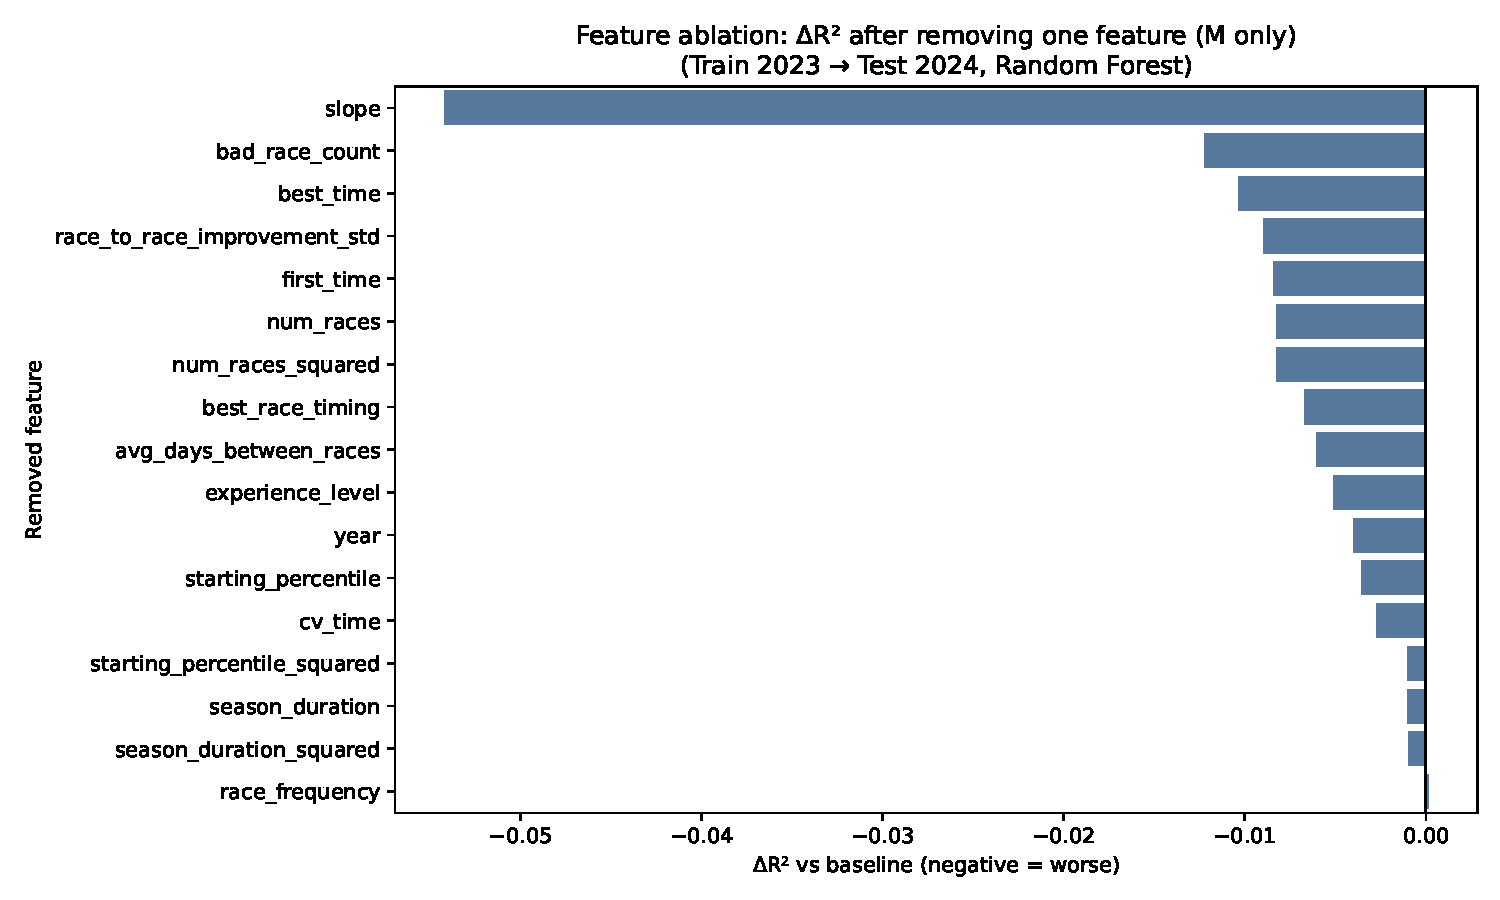
\includegraphics[width=\linewidth]{output/rq1/robustness_feature_ablation/feature_ablation_delta_r2_train_2023_test_2024_men.pdf}\\[0.3em]
    \small (a) Men
  \end{minipage}
  \hfill
  \begin{minipage}[t]{0.48\linewidth}
    \centering
    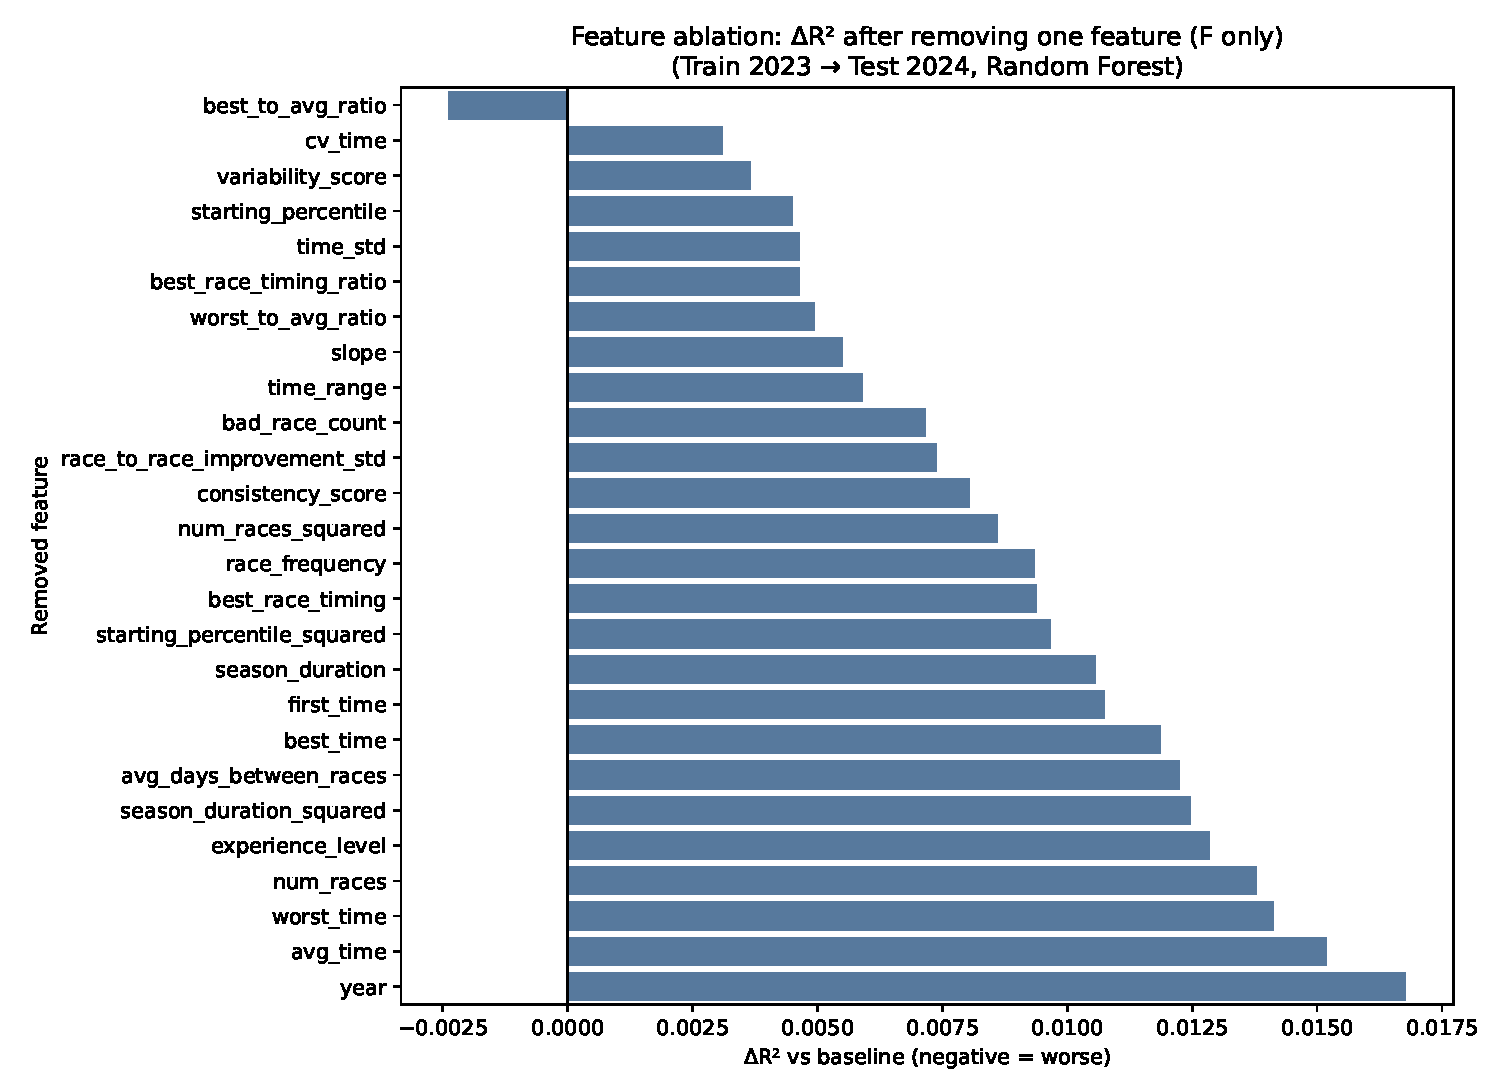
\includegraphics[width=\linewidth]{output/rq1/robustness_feature_ablation/feature_ablation_delta_r2_train_2023_test_2024_women.pdf}\\[0.3em]
    \small (b) Women
  \end{minipage}
  \caption{Feature ablation: $\Delta R^2$ relative to the sex-specific baseline when each feature is omitted (train 2023 $\rightarrow$ test 2024).}
  \label{fig:ablation-both}
\end{figure}

\begin{figure}[htbp]
  \centering
  \begin{minipage}[t]{0.48\linewidth}
    \centering
    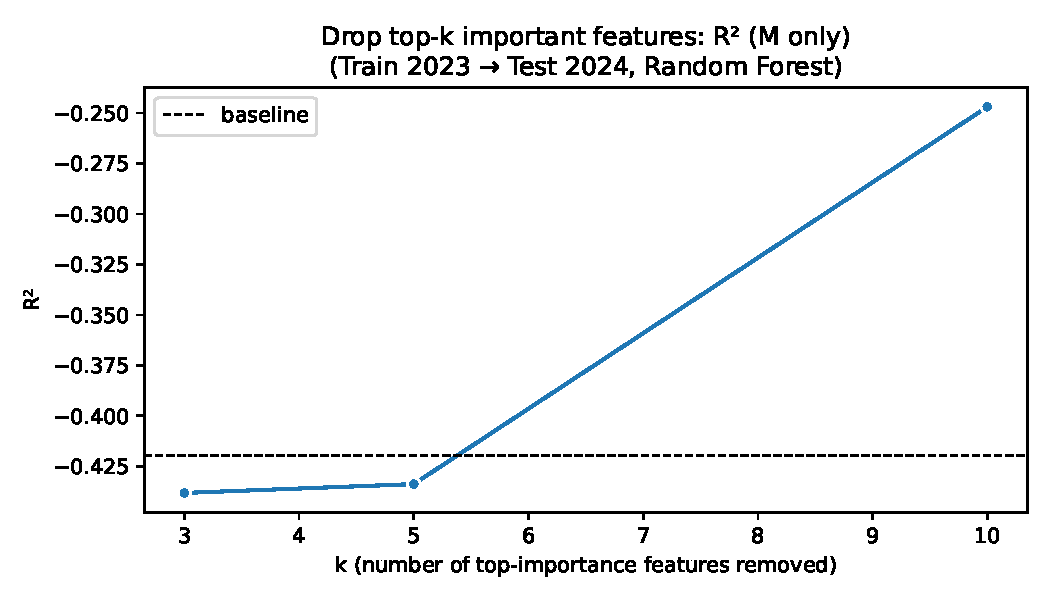
\includegraphics[width=\linewidth]{output/rq1/robustness_feature_ablation/feature_ablation_drop_topk_r2_train_2023_test_2024_men.pdf}\\[0.3em]
    \small (a) Men
  \end{minipage}
  \hfill
  \begin{minipage}[t]{0.48\linewidth}
    \centering
    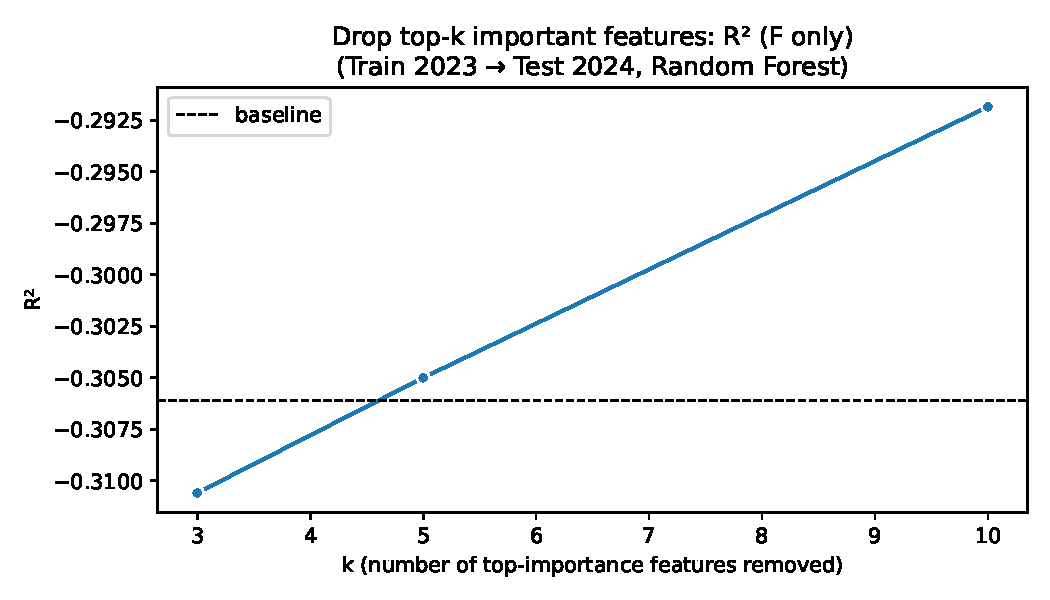
\includegraphics[width=\linewidth]{output/rq1/robustness_feature_ablation/feature_ablation_drop_topk_r2_train_2023_test_2024_women.pdf}\\[0.3em]
    \small (b) Women
  \end{minipage}
  \caption{Test $R^2$ after dropping the top-$k$ features by importance ranking (same split).}
  \label{fig:ablation-topk-both}
\end{figure}

\subsection{Sensitivity analysis}
\label{app:rq1_sensitivity}

We re-estimated the forest under alternative choices: tighter or wider clipping on \texttt{improvement\_rate}, dropping \texttt{last\_time}, dropping squared terms, dropping all raw time markers (\texttt{first\_time}, \texttt{last\_time}, \texttt{best\_time}, \texttt{worst\_time}, \texttt{avg\_time}), and varying \texttt{n\_estimators} $\in\{50,100,200\}$. On the primary split, men's test $R^2$ stayed near $0.819$ under the default $\pm 50$~s/day screen; removing \texttt{last\_time} changed $R^2$ by less than $+0.003$, and halving or doubling the forest size changed $| \Delta R^2|$ by at most $\approx 0.003$. Tighter clipping ($\pm 20$~s/day) raised men's apparent $R^2$ substantially ($\Delta R^2 \approx +0.11$) because extreme improvement-rate values were excluded. Women's baseline was $R^2=0.888$; removing \texttt{last\_time} gave $\Delta R^2 \approx -0.005$, and forest size had negligible effect ($|\Delta R^2| < 0.001$). Widening the improvement-rate band to $\pm 100$~s/day reduced women's $R^2$ by about $0.10$. Figure~\ref{fig:sensitivity-both} summarizes $\Delta R^2$ vs.\ baseline by scenario; Figure~\ref{fig:sensitivity-splits-both} shows $R^2$ across temporal splits (including train 2023 $\rightarrow$ test 2025 and train 2023+2024 $\rightarrow$ test 2025).

\begin{figure}[htbp]
  \centering
  \begin{minipage}[t]{0.48\linewidth}
    \centering
    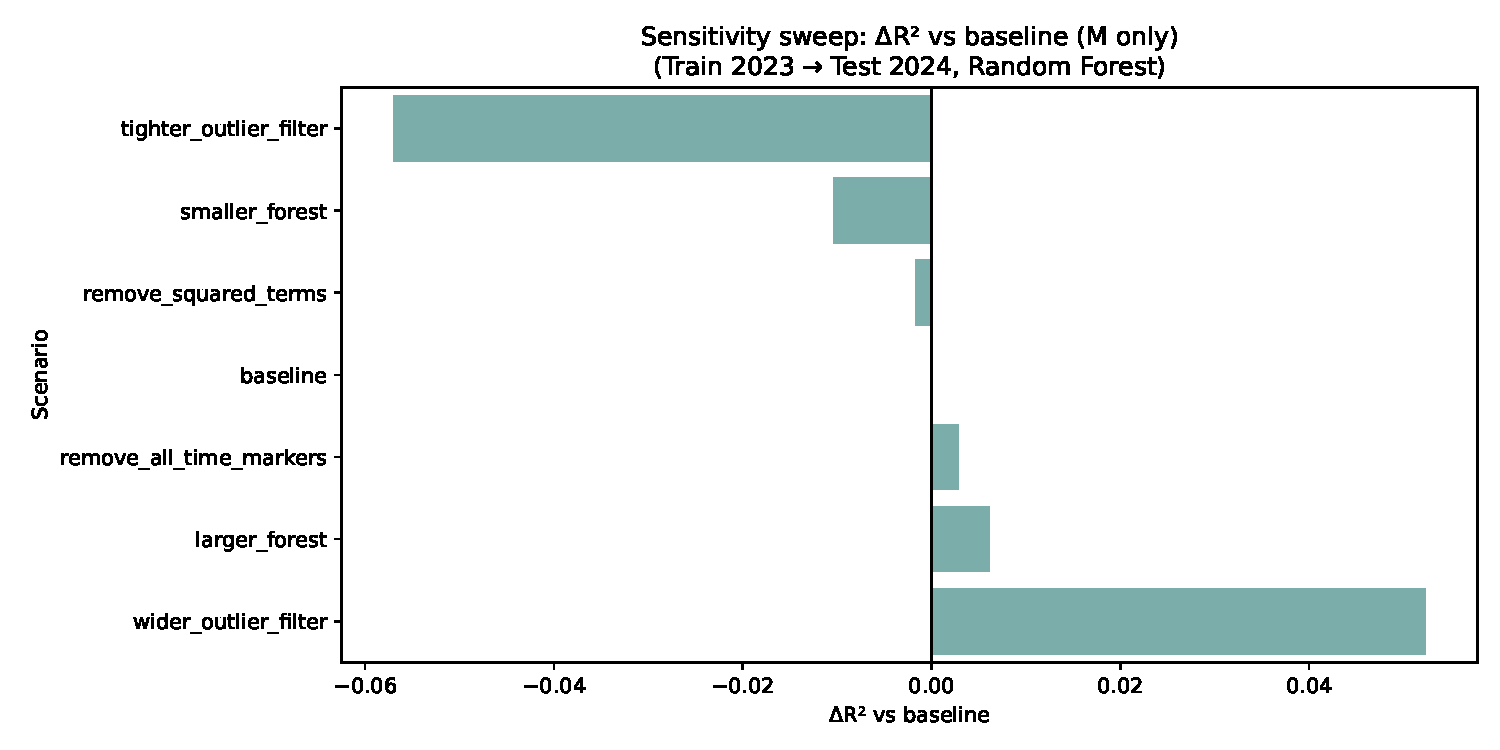
\includegraphics[width=\linewidth]{output/rq1/sensitivity_sweep/sensitivity_sweep_delta_r2_train_2023_test_2024_men.pdf}\\[0.3em]
    \small (a) Men
  \end{minipage}
  \hfill
  \begin{minipage}[t]{0.48\linewidth}
    \centering
    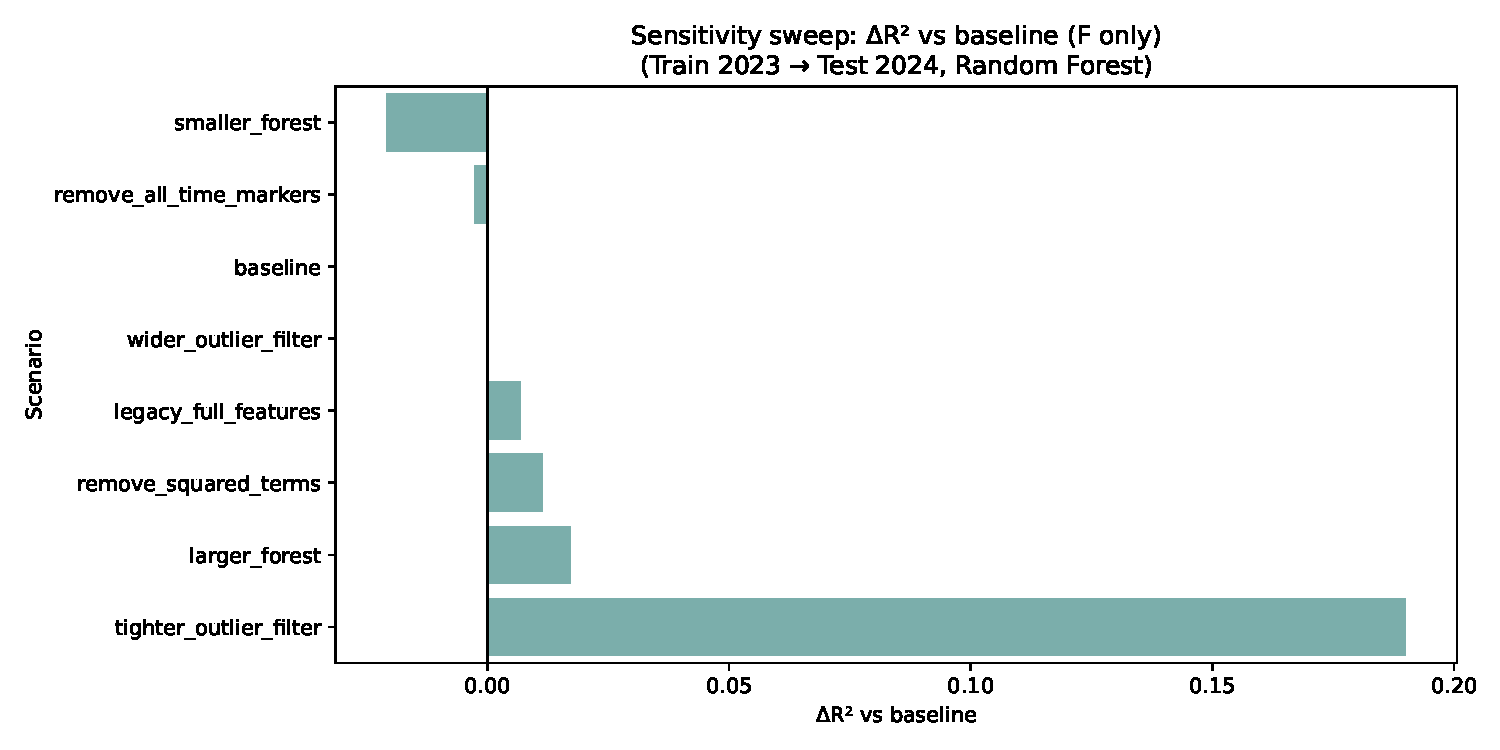
\includegraphics[width=\linewidth]{output/rq1/sensitivity_sweep/sensitivity_sweep_delta_r2_train_2023_test_2024_women.pdf}\\[0.3em]
    \small (b) Women
  \end{minipage}
  \caption{Sensitivity sweep: $\Delta R^2$ vs.\ the sex-specific baseline on the train-2023 $\rightarrow$ test-2024 split.}
  \label{fig:sensitivity-both}
\end{figure}

\begin{figure}[htbp]
  \centering
  \begin{minipage}[t]{0.48\linewidth}
    \centering
    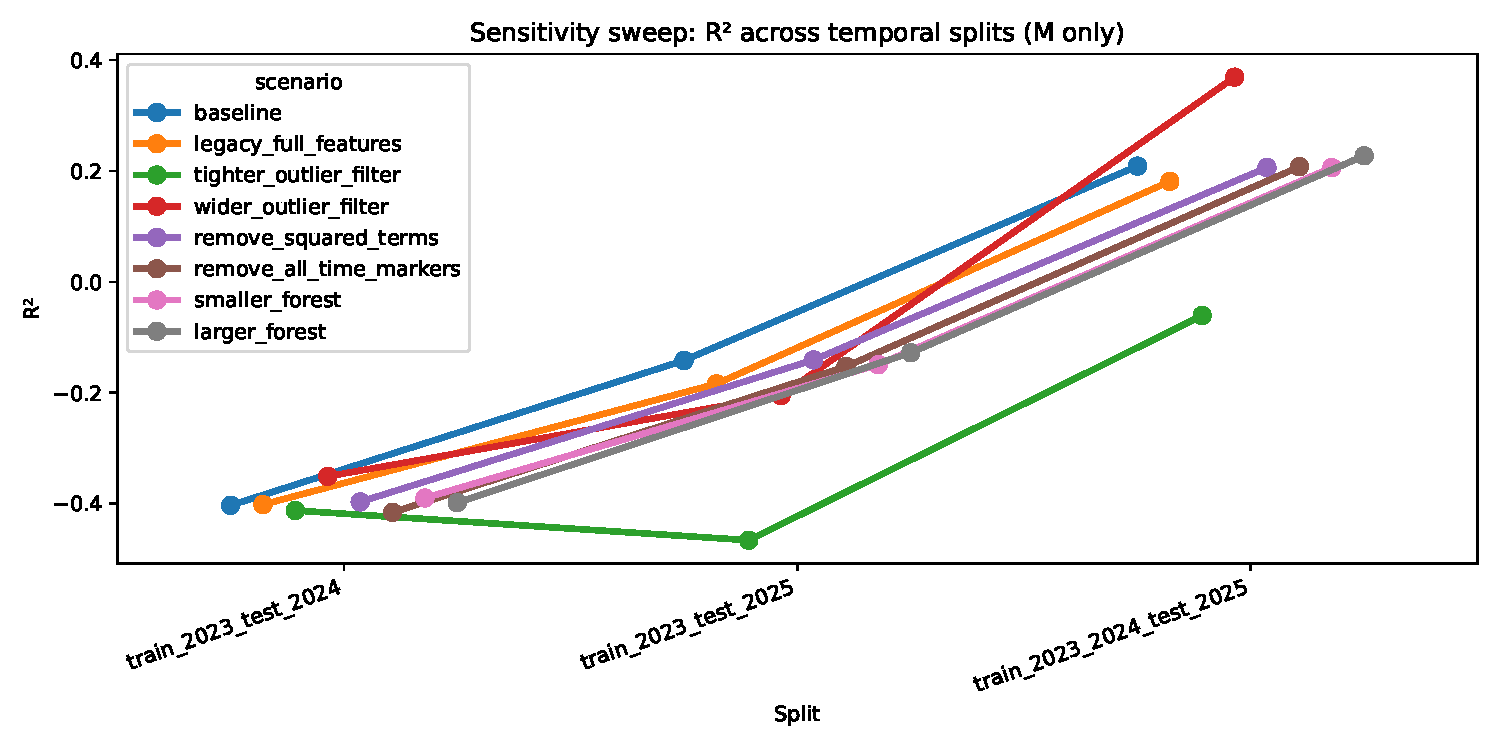
\includegraphics[width=\linewidth]{output/rq1/sensitivity_sweep/sensitivity_sweep_r2_across_splits_men.pdf}\\[0.3em]
    \small (a) Men
  \end{minipage}
  \hfill
  \begin{minipage}[t]{0.48\linewidth}
    \centering
    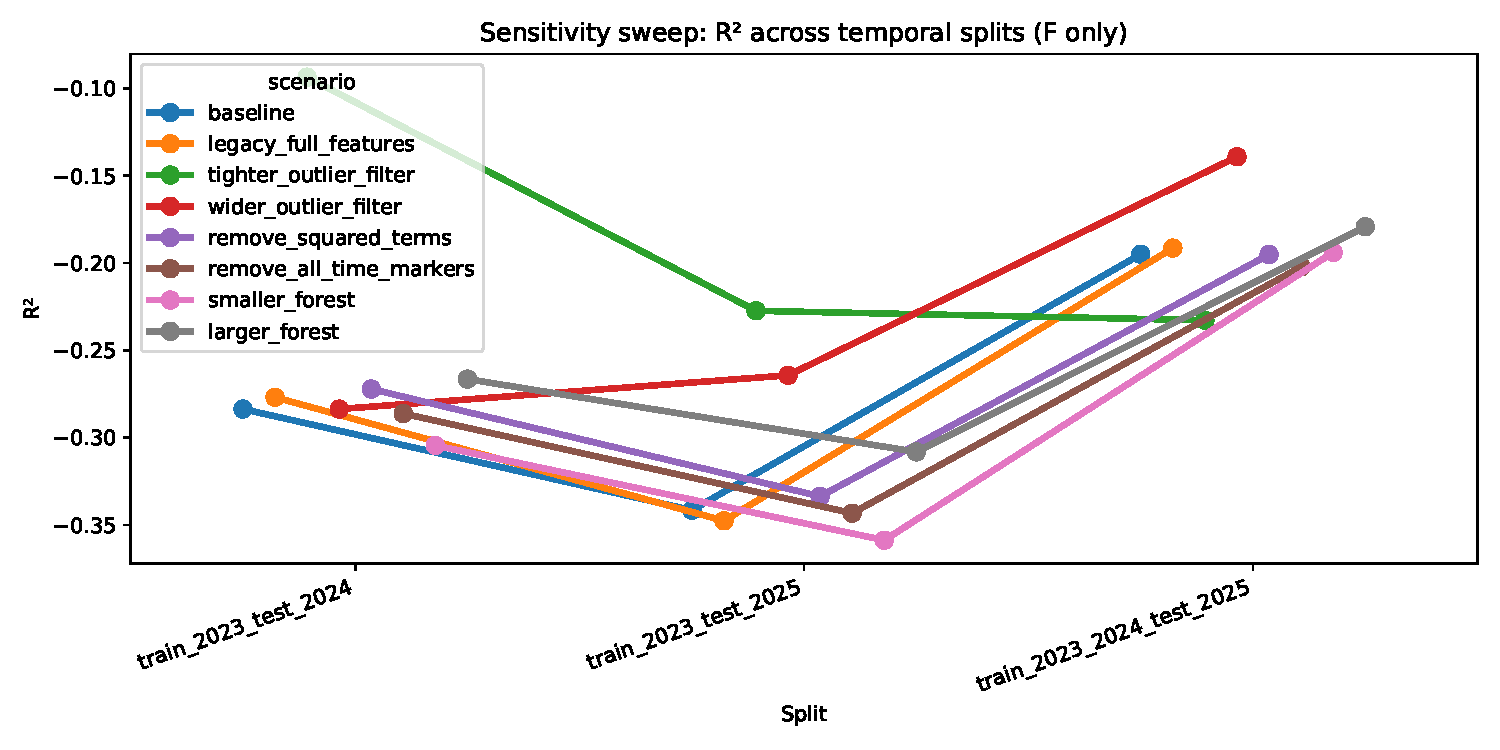
\includegraphics[width=\linewidth]{output/rq1/sensitivity_sweep/sensitivity_sweep_r2_across_splits_women.pdf}\\[0.3em]
    \small (b) Women
  \end{minipage}
  \caption{$R^2$ across temporal validation splits for each sensitivity scenario.}
  \label{fig:sensitivity-splits-both}
\end{figure}

\subsection{Mixed-effects explanatory models}
\label{app:rq1_mixed}

As an interpretable complement to the random forest, we fit linear mixed models with a random intercept for athlete. Fixed effects are $z$-scored \texttt{num\_races}, \texttt{season\_duration}, \texttt{starting\_percentile}, and calendar \texttt{year}, estimated separately within each sex. Coefficients are in seconds per day per one standard deviation increase in the predictor. Figure~\ref{fig:mixed-forest} plots fixed effects with 95\% confidence intervals; Table~\ref{tab:mixedlm-rq1} lists estimates.

\begin{figure}[htbp]
  \centering
  \begin{minipage}[t]{0.48\linewidth}
    \centering
    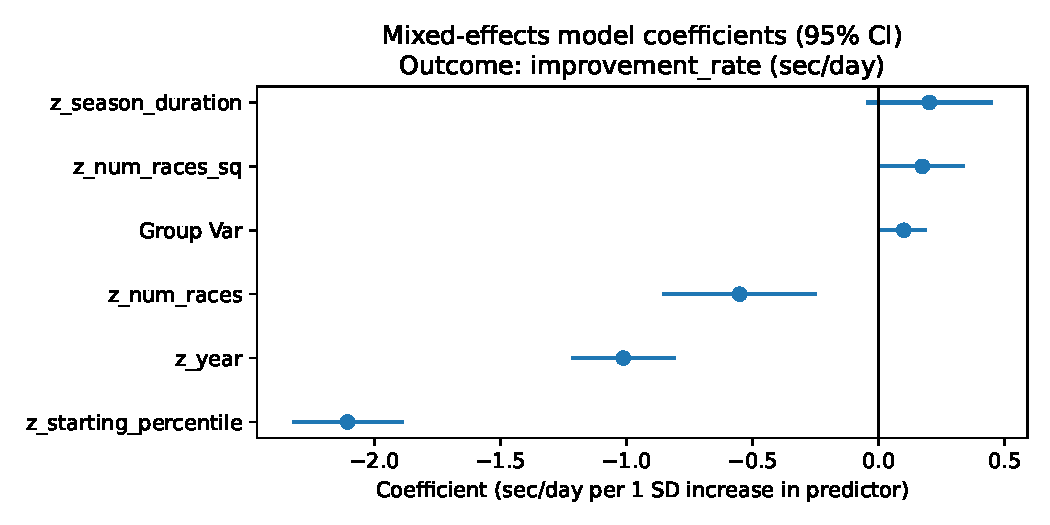
\includegraphics[width=\linewidth]{output/rq1/mixed_effects/mixedlm_coefficients_forest_men.pdf}\\[0.3em]
    \small (a) Men
  \end{minipage}
  \hfill
  \begin{minipage}[t]{0.48\linewidth}
    \centering
    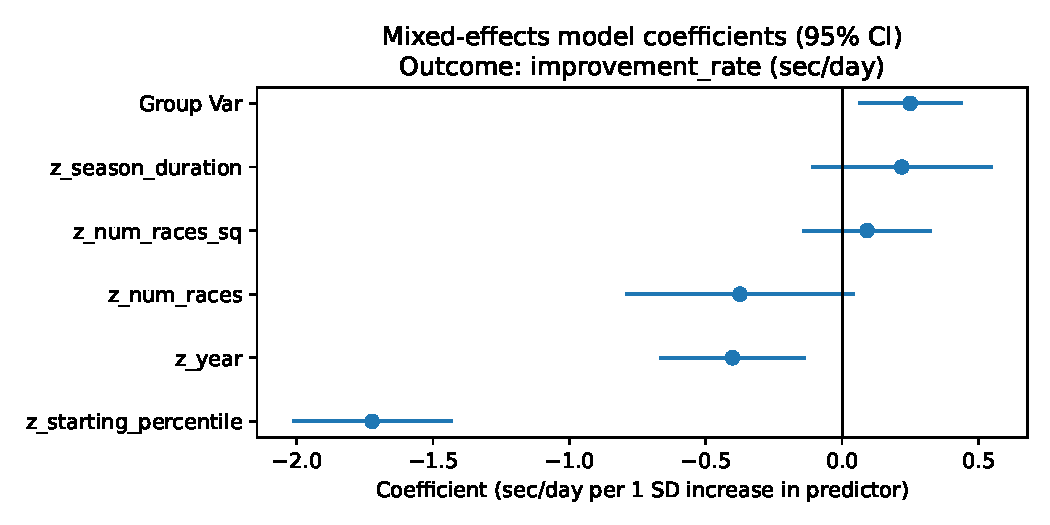
\includegraphics[width=\linewidth]{output/rq1/mixed_effects/mixedlm_coefficients_forest_women.pdf}\\[0.3em]
    \small (b) Women
  \end{minipage}
  \caption{Mixed-effects model: fixed-effect estimates with 95\% confidence intervals (outcome: \texttt{improvement\_rate}, seconds per day).}
  \label{fig:mixed-forest}
\end{figure}

\begin{table}[htbp]
  \centering
  \caption{Mixed-effects (MixedLM) fixed effects: estimate (seconds per day per 1 SD predictor), 95\% CI, two-sided $p$-value. Random intercept: athlete.}
  \label{tab:mixedlm-rq1}
  \begin{tabular}{l rrr rrr}
    \toprule
    & \multicolumn{3}{c}{Men} & \multicolumn{3}{c}{Women} \\
    \cmidrule(lr){2-4} \cmidrule(lr){5-7}
    Term & Est.\ & 95\% CI & $p$ & Est.\ & 95\% CI & $p$ \\
    \midrule
    Intercept
      & $-0.615$ & $[-0.781,\,-0.450]$ & $<0.001$
      & $-0.450$ & $[-0.654,\,-0.246]$ & $<0.001$ \\
    $z$\texttt{\_num\_races}
      & $-0.330$ & $[-0.568,\,-0.091]$ & $0.007$
      & $-0.160$ & $[-0.366,\ \ 0.046]$ & $0.128$ \\
    $z$\texttt{\_season\_duration}
      & $0.358$ & $[\ 0.187,\ \ 0.529]$ & $<0.001$
      & $0.282$ & $[-0.029,\ \ 0.592]$ & $0.075$ \\
    $z$\texttt{\_starting\_percentile}
      & $-1.188$ & $[-1.372,\,-1.004]$ & $<0.001$
      & $-0.676$ & $[-0.884,\,-0.468]$ & $<0.001$ \\
    $z$\texttt{\_year}
      & $-0.613$ & $[-0.769,\,-0.457]$ & $<0.001$
      & $-0.318$ & $[-0.556,\,-0.080]$ & $0.009$ \\
    \bottomrule
  \end{tabular}
\end{table}

\FloatBarrier
\section{Seasonal Participation Patterns}
\label{app:participation}

Understanding when athletes compete during the season provides important context for interpreting improvement patterns. Figure \ref{fig:weekly_participation} illustrates the weekly distribution of race participation by gender across the 2023-2025 seasons. This analysis reveals peak participation periods, seasonal timing of competitions, and gender-specific patterns in race scheduling. The visualization demonstrates that the number of runners racing increases throughout September and October. Yet, there is a decline in the number of people racing the week before regionals, which is either the week of October 21st or 28th, depending on the region and year.

\begin{figure}[htbp]
    \centering
    
\includegraphics[width=1\linewidth]{figures_for_sloan/weekly_participation_by_gender.pdf}
    \caption{Weekly Participation Patterns by Gender}
    \label{fig:weekly_participation}
\end{figure}
\FloatBarrier
\section{First-to-Fastest Race Improvement by Year}

Figures \ref{fig:men_overlay} and \ref{fig:women_overlay} provide year-by-year visualizations of the improvement patterns shown in Figure \ref{fig:combined_improvement} from the main text. These visualizations complement the combined analysis in Section 4.1.2 (Data Analytics) by revealing year-specific patterns and highlighting the consistency of our key finding across all three seasons.

\begin{figure}[htbp]
    \centering
    
\includegraphics[width=1\linewidth]{figures_for_sloan/combined_overlay_2023_2024_2025_mens.pdf}
    \caption{Men's Overlay Plots for 2023-2025}
    \label{fig:men_overlay}
\end{figure}

\begin{figure}[htbp]
    \centering
    
\includegraphics[width=1\linewidth]{figures_for_sloan/combined_overlay_2023_2024_2025_womens.pdf}
    \caption{Women's Overlay Plots for 2023-2025}
    \label{fig:women_overlay}
\end{figure}

\FloatBarrier

\section{Gender Specific Multi-Season Performance Analysis}
Figures \ref{fig:r2_men} and \ref{fig:r2_women} provide comprehensive visualizations of multi-season performance patterns that support the findings presented in Section 4.2 (Runners' Improvement Over Multiple Seasons). These comprehensive visualizations complement the gender comparison shown in Figure \ref{fig:gender_fast_times}.

\begin{figure}[htbp]
    \centering
    
\includegraphics[width=1\linewidth]{figures_for_sloan/rq2_comprehensive_men.pdf}
    \caption{Men's Multi-Season Performance Analysis}
    \label{fig:r2_men}
\end{figure}

\begin{figure}[htbp]
    \centering
    
\includegraphics[width=1\linewidth]{figures_for_sloan/rq2_comprehensive_women.pdf}
    \caption{Women's Multi-Season Performance Analysis}
    \label{fig:r2_women}
\end{figure}

\end{document}
